\documentclass[twoside]{book}

% Packages required by doxygen
\usepackage{calc}
\usepackage{doxygen}
\usepackage{graphicx}
\usepackage[utf8]{inputenc}
\usepackage{makeidx}
\usepackage{multicol}
\usepackage{multirow}
\usepackage{textcomp}
\usepackage[table]{xcolor}

% Font selection
\usepackage[T1]{fontenc}
\usepackage{mathptmx}
\usepackage[scaled=.90]{helvet}
\usepackage{courier}
\usepackage{amssymb}
\usepackage{sectsty}
\renewcommand{\familydefault}{\sfdefault}
\allsectionsfont{%
  \fontseries{bc}\selectfont%
  \color{darkgray}%
}
\renewcommand{\DoxyLabelFont}{%
  \fontseries{bc}\selectfont%
  \color{darkgray}%
}

% Page & text layout
\usepackage{geometry}
\geometry{%
  a4paper,%
  top=2.5cm,%
  bottom=2.5cm,%
  left=2.5cm,%
  right=2.5cm%
}
\tolerance=750
\hfuzz=15pt
\hbadness=750
\setlength{\emergencystretch}{15pt}
\setlength{\parindent}{0cm}
\setlength{\parskip}{0.2cm}
\makeatletter
\renewcommand{\paragraph}{%
  \@startsection{paragraph}{4}{0ex}{-1.0ex}{1.0ex}{%
    \normalfont\normalsize\bfseries\SS@parafont%
  }%
}
\renewcommand{\subparagraph}{%
  \@startsection{subparagraph}{5}{0ex}{-1.0ex}{1.0ex}{%
    \normalfont\normalsize\bfseries\SS@subparafont%
  }%
}
\makeatother

% Headers & footers
\usepackage{fancyhdr}
\pagestyle{fancyplain}
\fancyhead[LE]{\fancyplain{}{\bfseries\thepage}}
\fancyhead[CE]{\fancyplain{}{}}
\fancyhead[RE]{\fancyplain{}{\bfseries\leftmark}}
\fancyhead[LO]{\fancyplain{}{\bfseries\rightmark}}
\fancyhead[CO]{\fancyplain{}{}}
\fancyhead[RO]{\fancyplain{}{\bfseries\thepage}}
\fancyfoot[LE]{\fancyplain{}{}}
\fancyfoot[CE]{\fancyplain{}{}}
\fancyfoot[RE]{\fancyplain{}{\bfseries\scriptsize Generated on Fri May 2 2014 16\-:52\-:23 for redis3m by Doxygen }}
\fancyfoot[LO]{\fancyplain{}{\bfseries\scriptsize Generated on Fri May 2 2014 16\-:52\-:23 for redis3m by Doxygen }}
\fancyfoot[CO]{\fancyplain{}{}}
\fancyfoot[RO]{\fancyplain{}{}}
\renewcommand{\footrulewidth}{0.4pt}
\renewcommand{\chaptermark}[1]{%
  \markboth{#1}{}%
}
\renewcommand{\sectionmark}[1]{%
  \markright{\thesection\ #1}%
}

% Indices & bibliography
\usepackage{natbib}
\usepackage[titles]{tocloft}
\setcounter{tocdepth}{3}
\setcounter{secnumdepth}{5}
\makeindex

% Hyperlinks (required, but should be loaded last)
\usepackage{ifpdf}
\ifpdf
  \usepackage[pdftex,pagebackref=true]{hyperref}
\else
  \usepackage[ps2pdf,pagebackref=true]{hyperref}
\fi
\hypersetup{%
  colorlinks=true,%
  linkcolor=blue,%
  citecolor=blue,%
  unicode%
}

% Custom commands
\newcommand{\clearemptydoublepage}{%
  \newpage{\pagestyle{empty}\cleardoublepage}%
}


%===== C O N T E N T S =====

\begin{document}

% Titlepage & ToC
\hypersetup{pageanchor=false}
\pagenumbering{roman}
\begin{titlepage}
\vspace*{7cm}
\begin{center}%
{\Large redis3m \\[1ex]\large 1.\-0.\-0 }\\
\vspace*{1cm}
{\large Generated by Doxygen 1.8.6}\\
\vspace*{0.5cm}
{\small Fri May 2 2014 16:52:23}\\
\end{center}
\end{titlepage}
\clearemptydoublepage
\tableofcontents
\clearemptydoublepage
\pagenumbering{arabic}
\hypersetup{pageanchor=true}

%--- Begin generated contents ---
\chapter{redis3m}
\label{md__r_e_a_d_m_e}
\hypertarget{md__r_e_a_d_m_e}{}
\href{https://travis-ci.org/luca3m/redis3m}{\tt !\mbox{[}Build Status\mbox{]}(https\-://travis-\/ci.\-org/luca3m/redis3m.\-png?branch=master)}

A C++ \href{http://redis.io}{\tt Redis} driver, born to bring my experience using Redis and C++ on a opensource library.

\subsubsection*{Main goals}


\begin{DoxyEnumerate}
\item Provide a simple and efficient wrapper of \href{http://github.com/redis/hiredis}{\tt hiredis}, with C++ facilities like memory management
\item A connection pooling system, with support for high availability using sentinel
\item A set of useful patterns ready to use and composable with other code. For example \href{http://luca3m.me/2013/12/03/redis-scheduler.html}{\tt scheduler}, \href{http://github.com/soveran/ohm}{\tt orm}, counters or message queueing
\end{DoxyEnumerate}

\subsubsection*{Dependencies}

redis3m requires hiredis and boost libraries.

\subsubsection*{Install}

First step install all required dependencies, on a Debian system you can use\-:

```bash sudo apt-\/get install libmsgpack-\/dev libboost-\/thread-\/dev libboost-\/date-\/time-\/dev libboost-\/test-\/dev libboost-\/filesystem-\/dev libboost-\/system-\/dev libhiredis-\/dev cmake build-\/essential ```

Then checkout the code and compile it ```bash git clone \href{https://github.com/luca3m/redis3m}{\tt https\-://github.\-com/luca3m/redis3m} cd redis3m cmake make sudo make install ```

\subsubsection*{Documentation}

See \href{https://github.com/luca3m/redis3m/tree/master/examples}{\tt examples} directory for some examples, you can compile them with\-:

```bash g++ $<$example.\-cpp$>$ \$(pkg-\/config --cflags --libs redis3m) -\/o $<$example.\-bin$>$ ```

As reference you can read \href{https://github.com/luca3m/redis3m/tree/master/include}{\tt include} files, they are pretty simple and some of them are already documented with Doxygen.

\subsubsection*{Versioning}

This project uses \href{http://semver.org}{\tt semantic versioning}. In short words versions are named X.\-Y\mbox{[}.Z\mbox{]}. Changing X means break A\-P\-I changes, Y means new features without breaking old code, Z means bug fixing. 
\chapter{Hierarchical Index}
\section{Class Hierarchy}
This inheritance list is sorted roughly, but not completely, alphabetically\-:\begin{DoxyCompactList}
\item exception\begin{DoxyCompactList}
\item \contentsline{section}{redis3m\-:\-:exception}{\pageref{classredis3m_1_1exception}}{}
\end{DoxyCompactList}
\item \contentsline{section}{redis3m\-:\-:logging}{\pageref{classredis3m_1_1logging}}{}
\item \contentsline{section}{redis3m\-:\-:patterns\-:\-:model}{\pageref{classredis3m_1_1patterns_1_1model}}{}
\item noncopyable\begin{DoxyCompactList}
\item \contentsline{section}{redis3m\-:\-:connection}{\pageref{classredis3m_1_1connection}}{}
\item \contentsline{section}{redis3m\-:\-:connection\-\_\-pool}{\pageref{classredis3m_1_1connection__pool}}{}
\item \contentsline{section}{redis3m\-:\-:simple\-\_\-pool}{\pageref{classredis3m_1_1simple__pool}}{}
\end{DoxyCompactList}
\item \contentsline{section}{redis3m\-:\-:patterns\-:\-:orm$<$ Model $>$}{\pageref{classredis3m_1_1patterns_1_1orm}}{}
\item \contentsline{section}{redis3m\-:\-:reply}{\pageref{classredis3m_1_1reply}}{}
\item \contentsline{section}{redis3m\-:\-:patterns\-:\-:scheduler}{\pageref{classredis3m_1_1patterns_1_1scheduler}}{}
\item \contentsline{section}{redis3m\-:\-:patterns\-:\-:script\-\_\-exec}{\pageref{classredis3m_1_1patterns_1_1script__exec}}{}
\item \contentsline{section}{redis3m\-:\-:patterns\-:\-:simple\-\_\-obj\-\_\-store$<$ Model $>$}{\pageref{classredis3m_1_1patterns_1_1simple__obj__store}}{}
\end{DoxyCompactList}

\chapter{Class Index}
\section{Class List}
Here are the classes, structs, unions and interfaces with brief descriptions\-:\begin{DoxyCompactList}
\item\contentsline{section}{\hyperlink{classredis3m_1_1connection}{redis3m\-::connection} \\*The connection class, represent a connection to a Redis server }{\pageref{classredis3m_1_1connection}}{}
\item\contentsline{section}{\hyperlink{classredis3m_1_1connection__pool}{redis3m\-::connection\-\_\-pool} \\*Manages a connection pool, using a Redis Sentinel to get instaces ip, managing also failover }{\pageref{classredis3m_1_1connection__pool}}{}
\item\contentsline{section}{\hyperlink{classredis3m_1_1exception}{redis3m\-::exception} }{\pageref{classredis3m_1_1exception}}{}
\item\contentsline{section}{\hyperlink{classredis3m_1_1logging}{redis3m\-::logging} }{\pageref{classredis3m_1_1logging}}{}
\item\contentsline{section}{\hyperlink{classredis3m_1_1patterns_1_1model}{redis3m\-::patterns\-::model} \\*Class useful to define models used by \hyperlink{classredis3m_1_1patterns_1_1orm}{orm} and \hyperlink{classredis3m_1_1patterns_1_1simple__obj__store}{simple\-\_\-obj\-\_\-store}. R\-E\-D\-I\-S3\-M\-\_\-\-M\-O\-D\-E\-L\-\_\-\-R\-O\-\_\-\-A\-T\-T\-R\-I\-B\-U\-T\-E(type, name) macro defines automatically an attribute with a public getter. All fields need to be serialized to a std\-::map$<$std\-::string, std\-::string$>$. Model class contains various helpers to to that easily }{\pageref{classredis3m_1_1patterns_1_1model}}{}
\item\contentsline{section}{\hyperlink{classredis3m_1_1patterns_1_1orm}{redis3m\-::patterns\-::orm$<$ Model $>$} \\*Object-\/\-Redis-\/\-Mapper is a convenient pattern to store object on Redis. Useful when you need classic C\-R\-U\-D operations. It's compatible and inspired by \href{http://github.com/soveran/ohm}{\tt http\-://github.\-com/soveran/ohm}. Data can be indexed and it supports also uniques. To use it make a subclass of \hyperlink{classredis3m_1_1patterns_1_1model}{model} to model your attribute and use it to fill orm template parameter }{\pageref{classredis3m_1_1patterns_1_1orm}}{}
\item\contentsline{section}{\hyperlink{classredis3m_1_1reply}{redis3m\-::reply} \\*Represent a reply received from redis server }{\pageref{classredis3m_1_1reply}}{}
\item\contentsline{section}{\hyperlink{classredis3m_1_1patterns_1_1scheduler}{redis3m\-::patterns\-::scheduler} \\*A scheduler pattern, can be useful to manage \char`\"{}jobs\char`\"{} that needs to be run at a given time. It's fault tolerant and scalable. Multiple workers can be dispatched and jobs will be executed only once. See \href{http://luca3m.me/2013/12/03/redis-scheduler.html}{\tt http\-://luca3m.\-me/2013/12/03/redis-\/scheduler.\-html} for other infos }{\pageref{classredis3m_1_1patterns_1_1scheduler}}{}
\item\contentsline{section}{\hyperlink{classredis3m_1_1patterns_1_1script__exec}{redis3m\-::patterns\-::script\-\_\-exec} \\*Helps to run Lua scripts on a Redis instance. It will take care to use E\-V\-A\-L\-S\-H\-A to optimize performance and then E\-V\-A\-L if the script is not yet available on Redis server. See \href{http://redis.io/commands/eval}{\tt http\-://redis.\-io/commands/eval} for other infos }{\pageref{classredis3m_1_1patterns_1_1script__exec}}{}
\item\contentsline{section}{\hyperlink{classredis3m_1_1patterns_1_1simple__obj__store}{redis3m\-::patterns\-::simple\-\_\-obj\-\_\-store$<$ Model $>$} \\*Simple object storage, ready to use save, find and remove of \hyperlink{classredis3m_1_1patterns_1_1model}{model} classes. id management is not provided }{\pageref{classredis3m_1_1patterns_1_1simple__obj__store}}{}
\item\contentsline{section}{\hyperlink{classredis3m_1_1simple__pool}{redis3m\-::simple\-\_\-pool} \\*Manages a pool of connections to a single Redis server }{\pageref{classredis3m_1_1simple__pool}}{}
\end{DoxyCompactList}

\chapter{Class Documentation}
\hypertarget{classredis3m_1_1connection}{\section{redis3m\-:\-:connection Class Reference}
\label{classredis3m_1_1connection}\index{redis3m\-::connection@{redis3m\-::connection}}
}


The connection class, represent a connection to a Redis server.  




{\ttfamily \#include $<$connection.\-h$>$}

Inheritance diagram for redis3m\-:\-:connection\-:\begin{figure}[H]
\begin{center}
\leavevmode
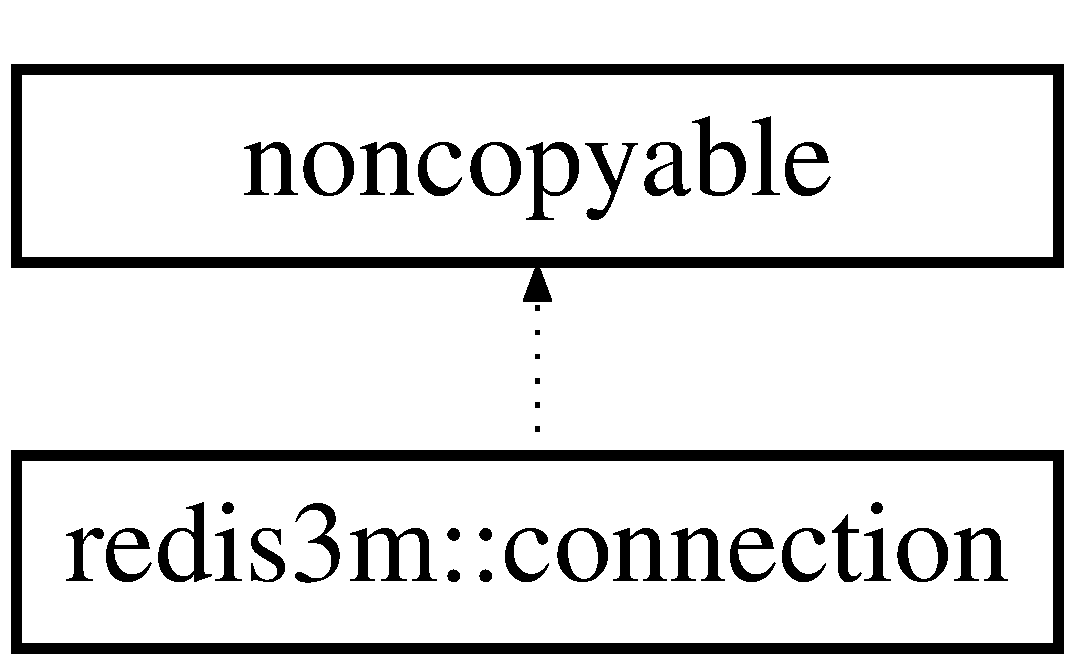
\includegraphics[height=2.000000cm]{classredis3m_1_1connection}
\end{center}
\end{figure}
\subsection*{Public Types}
\begin{DoxyCompactItemize}
\item 
enum {\bfseries role\-\_\-t} \{ {\bfseries A\-N\-Y} = 0, 
{\bfseries M\-A\-S\-T\-E\-R} = 1, 
{\bfseries S\-L\-A\-V\-E} = 2
 \}
\item 
\hypertarget{classredis3m_1_1connection_a6e3fffb8c2b60128baf8ef0e9b78cbd3}{typedef boost\-::shared\-\_\-ptr\\*
$<$ \hyperlink{classredis3m_1_1connection}{connection} $>$ {\bfseries ptr\-\_\-t}}\label{classredis3m_1_1connection_a6e3fffb8c2b60128baf8ef0e9b78cbd3}

\end{DoxyCompactItemize}
\subsection*{Public Member Functions}
\begin{DoxyCompactItemize}
\item 
\hypertarget{classredis3m_1_1connection_a8ab5fc0ed61431b65220d2b389e8357e}{bool {\bfseries is\-\_\-valid} ()}\label{classredis3m_1_1connection_a8ab5fc0ed61431b65220d2b389e8357e}

\item 
void \hyperlink{classredis3m_1_1connection_a308ac2576c2dd1c8ce6e97c4572c86f5}{append} (const std\-::vector$<$ std\-::string $>$ \&args)
\begin{DoxyCompactList}\small\item\em Append a command to Redis server. \end{DoxyCompactList}\item 
\hyperlink{classredis3m_1_1reply}{reply} \hyperlink{classredis3m_1_1connection_a0c01abebb9be6368d3d159d30522e8c2}{get\-\_\-reply} ()
\begin{DoxyCompactList}\small\item\em Get a reply from server, blocking call if no reply is ready. \end{DoxyCompactList}\item 
std\-::vector$<$ \hyperlink{classredis3m_1_1reply}{reply} $>$ \hyperlink{classredis3m_1_1connection_a4a346751b7b4f47f5a5d702ad10b2490}{get\-\_\-replies} (unsigned int count)
\begin{DoxyCompactList}\small\item\em Get specific count of replies requested, blocking if they are not ready yet. \end{DoxyCompactList}\item 
\hyperlink{classredis3m_1_1reply}{reply} \hyperlink{classredis3m_1_1connection_ab2690e664a0f0bd4647be5b0f07f988b}{run} (const std\-::vector$<$ std\-::string $>$ \&args)
\begin{DoxyCompactList}\small\item\em Utility to call append and then get\-\_\-reply together. \end{DoxyCompactList}\item 
redis\-Context $\ast$ \hyperlink{classredis3m_1_1connection_a7c583cf358ea3d4b20583670280072ae}{c\-\_\-ptr} ()
\begin{DoxyCompactList}\small\item\em Returns raw ptr to hiredis library connection. Use it with caution and pay attention on memory management. \end{DoxyCompactList}\end{DoxyCompactItemize}
\subsection*{Static Public Member Functions}
\begin{DoxyCompactItemize}
\item 
static ptr\-\_\-t \hyperlink{classredis3m_1_1connection_a367251876cd720fe0a58727e2c8d202c}{create} (const std\-::string \&host=\char`\"{}localhost\char`\"{}, const unsigned int port=6379)
\begin{DoxyCompactList}\small\item\em Create and open a new connection. \end{DoxyCompactList}\end{DoxyCompactItemize}
\subsection*{Friends}
\begin{DoxyCompactItemize}
\item 
\hypertarget{classredis3m_1_1connection_accac599643e0a8c900f765dcf4026344}{class {\bfseries connection\-\_\-pool}}\label{classredis3m_1_1connection_accac599643e0a8c900f765dcf4026344}

\end{DoxyCompactItemize}


\subsection{Detailed Description}
The connection class, represent a connection to a Redis server. 

\subsection{Member Function Documentation}
\hypertarget{classredis3m_1_1connection_a308ac2576c2dd1c8ce6e97c4572c86f5}{\index{redis3m\-::connection@{redis3m\-::connection}!append@{append}}
\index{append@{append}!redis3m::connection@{redis3m\-::connection}}
\subsubsection[{append}]{\setlength{\rightskip}{0pt plus 5cm}void connection\-::append (
\begin{DoxyParamCaption}
\item[{const std\-::vector$<$ std\-::string $>$ \&}]{args}
\end{DoxyParamCaption}
)}}\label{classredis3m_1_1connection_a308ac2576c2dd1c8ce6e97c4572c86f5}


Append a command to Redis server. 


\begin{DoxyParams}{Parameters}
{\em args} & vector with args, example \mbox{[} \char`\"{}\-S\-E\-T\char`\"{}, \char`\"{}foo\char`\"{}, \char`\"{}bar\char`\"{} \mbox{]} \\
\hline
\end{DoxyParams}
\hypertarget{classredis3m_1_1connection_a7c583cf358ea3d4b20583670280072ae}{\index{redis3m\-::connection@{redis3m\-::connection}!c\-\_\-ptr@{c\-\_\-ptr}}
\index{c\-\_\-ptr@{c\-\_\-ptr}!redis3m::connection@{redis3m\-::connection}}
\subsubsection[{c\-\_\-ptr}]{\setlength{\rightskip}{0pt plus 5cm}redis\-Context$\ast$ redis3m\-::connection\-::c\-\_\-ptr (
\begin{DoxyParamCaption}
{}
\end{DoxyParamCaption}
)\hspace{0.3cm}{\ttfamily [inline]}}}\label{classredis3m_1_1connection_a7c583cf358ea3d4b20583670280072ae}


Returns raw ptr to hiredis library connection. Use it with caution and pay attention on memory management. 

\begin{DoxyReturn}{Returns}

\end{DoxyReturn}
\hypertarget{classredis3m_1_1connection_a367251876cd720fe0a58727e2c8d202c}{\index{redis3m\-::connection@{redis3m\-::connection}!create@{create}}
\index{create@{create}!redis3m::connection@{redis3m\-::connection}}
\subsubsection[{create}]{\setlength{\rightskip}{0pt plus 5cm}static ptr\-\_\-t redis3m\-::connection\-::create (
\begin{DoxyParamCaption}
\item[{const std\-::string \&}]{host = {\ttfamily \char`\"{}localhost\char`\"{}}, }
\item[{const unsigned int}]{port = {\ttfamily 6379}}
\end{DoxyParamCaption}
)\hspace{0.3cm}{\ttfamily [inline]}, {\ttfamily [static]}}}\label{classredis3m_1_1connection_a367251876cd720fe0a58727e2c8d202c}


Create and open a new connection. 


\begin{DoxyParams}{Parameters}
{\em host} & hostname or ip of redis server, default localhost \\
\hline
{\em port} & port of redis server, default\-: 6379 \\
\hline
\end{DoxyParams}
\begin{DoxyReturn}{Returns}

\end{DoxyReturn}
\hypertarget{classredis3m_1_1connection_a4a346751b7b4f47f5a5d702ad10b2490}{\index{redis3m\-::connection@{redis3m\-::connection}!get\-\_\-replies@{get\-\_\-replies}}
\index{get\-\_\-replies@{get\-\_\-replies}!redis3m::connection@{redis3m\-::connection}}
\subsubsection[{get\-\_\-replies}]{\setlength{\rightskip}{0pt plus 5cm}std\-::vector$<$ {\bf reply} $>$ connection\-::get\-\_\-replies (
\begin{DoxyParamCaption}
\item[{unsigned int}]{count}
\end{DoxyParamCaption}
)}}\label{classredis3m_1_1connection_a4a346751b7b4f47f5a5d702ad10b2490}


Get specific count of replies requested, blocking if they are not ready yet. 


\begin{DoxyParams}{Parameters}
{\em count} & \\
\hline
\end{DoxyParams}
\begin{DoxyReturn}{Returns}

\end{DoxyReturn}
\hypertarget{classredis3m_1_1connection_a0c01abebb9be6368d3d159d30522e8c2}{\index{redis3m\-::connection@{redis3m\-::connection}!get\-\_\-reply@{get\-\_\-reply}}
\index{get\-\_\-reply@{get\-\_\-reply}!redis3m::connection@{redis3m\-::connection}}
\subsubsection[{get\-\_\-reply}]{\setlength{\rightskip}{0pt plus 5cm}{\bf reply} connection\-::get\-\_\-reply (
\begin{DoxyParamCaption}
{}
\end{DoxyParamCaption}
)}}\label{classredis3m_1_1connection_a0c01abebb9be6368d3d159d30522e8c2}


Get a reply from server, blocking call if no reply is ready. 

\begin{DoxyReturn}{Returns}
reply object 
\end{DoxyReturn}
\hypertarget{classredis3m_1_1connection_ab2690e664a0f0bd4647be5b0f07f988b}{\index{redis3m\-::connection@{redis3m\-::connection}!run@{run}}
\index{run@{run}!redis3m::connection@{redis3m\-::connection}}
\subsubsection[{run}]{\setlength{\rightskip}{0pt plus 5cm}{\bf reply} redis3m\-::connection\-::run (
\begin{DoxyParamCaption}
\item[{const std\-::vector$<$ std\-::string $>$ \&}]{args}
\end{DoxyParamCaption}
)\hspace{0.3cm}{\ttfamily [inline]}}}\label{classredis3m_1_1connection_ab2690e664a0f0bd4647be5b0f07f988b}


Utility to call append and then get\-\_\-reply together. 


\begin{DoxyParams}{Parameters}
{\em args} & same as \hyperlink{classredis3m_1_1connection_a308ac2576c2dd1c8ce6e97c4572c86f5}{append()} \\
\hline
\end{DoxyParams}
\begin{DoxyReturn}{Returns}
reply object 
\end{DoxyReturn}


The documentation for this class was generated from the following files\-:\begin{DoxyCompactItemize}
\item 
include/redis3m/connection.\-h\item 
src/connection.\-cpp\end{DoxyCompactItemize}

\hypertarget{classredis3m_1_1connection__pool}{\section{redis3m\-:\-:connection\-\_\-pool Class Reference}
\label{classredis3m_1_1connection__pool}\index{redis3m\-::connection\-\_\-pool@{redis3m\-::connection\-\_\-pool}}
}


Manages a connection pool, using a Redis Sentinel to get instaces ip, managing also failover.  




{\ttfamily \#include $<$connection\-\_\-pool.\-h$>$}

Inheritance diagram for redis3m\-:\-:connection\-\_\-pool\-:\begin{figure}[H]
\begin{center}
\leavevmode
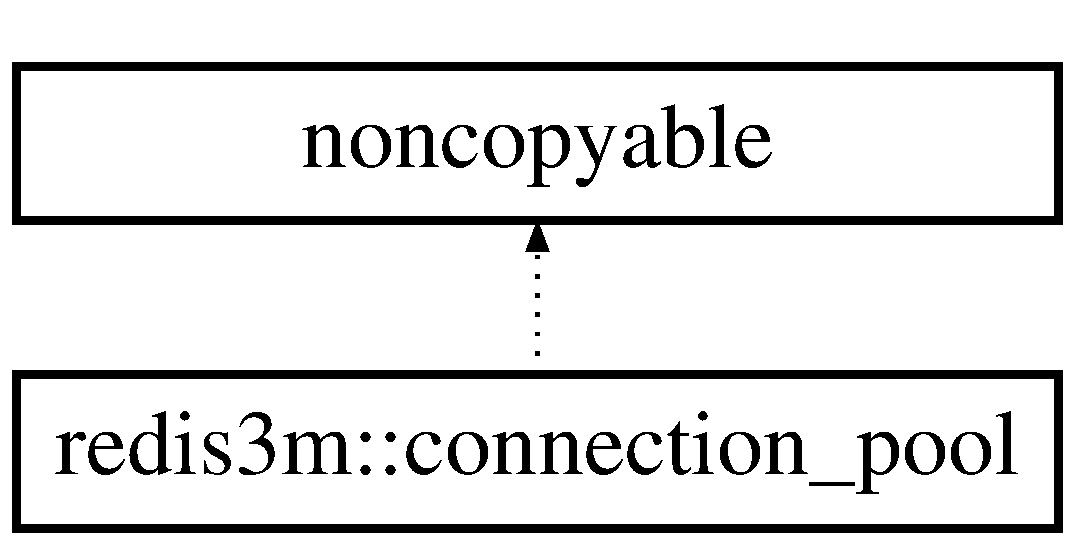
\includegraphics[height=2.000000cm]{classredis3m_1_1connection__pool}
\end{center}
\end{figure}
\subsection*{Public Types}
\begin{DoxyCompactItemize}
\item 
\hypertarget{classredis3m_1_1connection__pool_ac4288428ed17ad5b4a2247d859d99082}{typedef boost\-::shared\-\_\-ptr\\*
$<$ \hyperlink{classredis3m_1_1connection__pool}{connection\-\_\-pool} $>$ {\bfseries ptr\-\_\-t}}\label{classredis3m_1_1connection__pool_ac4288428ed17ad5b4a2247d859d99082}

\end{DoxyCompactItemize}
\subsection*{Public Member Functions}
\begin{DoxyCompactItemize}
\item 
connection\-::ptr\-\_\-t \hyperlink{classredis3m_1_1connection__pool_a64b7414a59f5ebb741f60f15269239cb}{get} (connection\-::role\-\_\-t type=connection\-::\-M\-A\-S\-T\-E\-R)
\begin{DoxyCompactList}\small\item\em Ask for a connection. \end{DoxyCompactList}\item 
void \hyperlink{classredis3m_1_1connection__pool_af98d6557618b0b3f2fb98a16f1248884}{put} (connection\-::ptr\-\_\-t conn)
\begin{DoxyCompactList}\small\item\em Put a connection again on pool for reuse, pay attention to insert only connection created from the same pool. Otherwise unpexpected behaviours can happen. \end{DoxyCompactList}\item 
{\footnotesize template$<$typename Ret $>$ }\\Ret \hyperlink{classredis3m_1_1connection__pool_a4bbb7ca50a001ae9f3917def5007d0d7}{run\-\_\-with\-\_\-connection} (boost\-::function$<$ Ret(connection\-::ptr\-\_\-t)$>$ f, connection\-::role\-\_\-t conn\-\_\-type=connection\-::\-M\-A\-S\-T\-E\-R, unsigned int retries=5)
\begin{DoxyCompactList}\small\item\em Execute a block of code passing a connection\-::ptr\-\_\-t if something fails, like broken connection, it will automatically retry with an another one. \end{DoxyCompactList}\item 
void \hyperlink{classredis3m_1_1connection__pool_a6d42ddca75faeb5c33f9d3bf04f44c5b}{set\-\_\-database} (unsigned int value)
\begin{DoxyCompactList}\small\item\em Set a database to use on every new connection object created by the pool. \end{DoxyCompactList}\item 
\hypertarget{classredis3m_1_1connection__pool_ab57e4c5fd3b58fb7e2242825b7868478}{{\footnotesize template$<$$>$ }\\void {\bfseries run\-\_\-with\-\_\-connection} (boost\-::function$<$ void(connection\-::ptr\-\_\-t)$>$ f, connection\-::role\-\_\-t conn\-\_\-type, unsigned int retries)}\label{classredis3m_1_1connection__pool_ab57e4c5fd3b58fb7e2242825b7868478}

\end{DoxyCompactItemize}
\subsection*{Static Public Member Functions}
\begin{DoxyCompactItemize}
\item 
static ptr\-\_\-t \hyperlink{classredis3m_1_1connection__pool_a75ee0b238816effb57301c5cbae720b4}{create} (const std\-::string \&sentinel\-\_\-host, const std\-::string \&master\-\_\-name, unsigned int sentinel\-\_\-port=26379)
\begin{DoxyCompactList}\small\item\em Create a new \hyperlink{classredis3m_1_1connection__pool}{connection\-\_\-pool}. \end{DoxyCompactList}\end{DoxyCompactItemize}


\subsection{Detailed Description}
Manages a connection pool, using a Redis Sentinel to get instaces ip, managing also failover. 

\subsection{Member Function Documentation}
\hypertarget{classredis3m_1_1connection__pool_a75ee0b238816effb57301c5cbae720b4}{\index{redis3m\-::connection\-\_\-pool@{redis3m\-::connection\-\_\-pool}!create@{create}}
\index{create@{create}!redis3m::connection_pool@{redis3m\-::connection\-\_\-pool}}
\subsubsection[{create}]{\setlength{\rightskip}{0pt plus 5cm}static ptr\-\_\-t redis3m\-::connection\-\_\-pool\-::create (
\begin{DoxyParamCaption}
\item[{const std\-::string \&}]{sentinel\-\_\-host, }
\item[{const std\-::string \&}]{master\-\_\-name, }
\item[{unsigned int}]{sentinel\-\_\-port = {\ttfamily 26379}}
\end{DoxyParamCaption}
)\hspace{0.3cm}{\ttfamily [inline]}, {\ttfamily [static]}}}\label{classredis3m_1_1connection__pool_a75ee0b238816effb57301c5cbae720b4}


Create a new \hyperlink{classredis3m_1_1connection__pool}{connection\-\_\-pool}. 


\begin{DoxyParams}{Parameters}
{\em sentinel\-\_\-host} & Can be a single host or a list separate by commas, if an host has multiple I\-Ps, \hyperlink{classredis3m_1_1connection__pool}{connection\-\_\-pool} tries all of them \\
\hline
{\em master\-\_\-name} & Master to lookup \\
\hline
{\em sentinel\-\_\-port} & Sentinel port, default 26379 \\
\hline
\end{DoxyParams}
\begin{DoxyReturn}{Returns}

\end{DoxyReturn}
\hypertarget{classredis3m_1_1connection__pool_a64b7414a59f5ebb741f60f15269239cb}{\index{redis3m\-::connection\-\_\-pool@{redis3m\-::connection\-\_\-pool}!get@{get}}
\index{get@{get}!redis3m::connection_pool@{redis3m\-::connection\-\_\-pool}}
\subsubsection[{get}]{\setlength{\rightskip}{0pt plus 5cm}connection\-::ptr\-\_\-t connection\-\_\-pool\-::get (
\begin{DoxyParamCaption}
\item[{connection\-::role\-\_\-t}]{type = {\ttfamily connection\-:\-:MASTER}}
\end{DoxyParamCaption}
)}}\label{classredis3m_1_1connection__pool_a64b7414a59f5ebb741f60f15269239cb}


Ask for a connection. 


\begin{DoxyParams}{Parameters}
{\em type} & Specify the type required, Master, Slave or Any \\
\hline
\end{DoxyParams}
\begin{DoxyReturn}{Returns}
a valid connection object 
\end{DoxyReturn}
\hypertarget{classredis3m_1_1connection__pool_af98d6557618b0b3f2fb98a16f1248884}{\index{redis3m\-::connection\-\_\-pool@{redis3m\-::connection\-\_\-pool}!put@{put}}
\index{put@{put}!redis3m::connection_pool@{redis3m\-::connection\-\_\-pool}}
\subsubsection[{put}]{\setlength{\rightskip}{0pt plus 5cm}void connection\-\_\-pool\-::put (
\begin{DoxyParamCaption}
\item[{connection\-::ptr\-\_\-t}]{conn}
\end{DoxyParamCaption}
)}}\label{classredis3m_1_1connection__pool_af98d6557618b0b3f2fb98a16f1248884}


Put a connection again on pool for reuse, pay attention to insert only connection created from the same pool. Otherwise unpexpected behaviours can happen. 


\begin{DoxyParams}{Parameters}
{\em conn} & \\
\hline
\end{DoxyParams}
\hypertarget{classredis3m_1_1connection__pool_a4bbb7ca50a001ae9f3917def5007d0d7}{\index{redis3m\-::connection\-\_\-pool@{redis3m\-::connection\-\_\-pool}!run\-\_\-with\-\_\-connection@{run\-\_\-with\-\_\-connection}}
\index{run\-\_\-with\-\_\-connection@{run\-\_\-with\-\_\-connection}!redis3m::connection_pool@{redis3m\-::connection\-\_\-pool}}
\subsubsection[{run\-\_\-with\-\_\-connection}]{\setlength{\rightskip}{0pt plus 5cm}template$<$typename Ret $>$ Ret redis3m\-::connection\-\_\-pool\-::run\-\_\-with\-\_\-connection (
\begin{DoxyParamCaption}
\item[{boost\-::function$<$ Ret(connection\-::ptr\-\_\-t)$>$}]{f, }
\item[{connection\-::role\-\_\-t}]{conn\-\_\-type = {\ttfamily connection\-:\-:MASTER}, }
\item[{unsigned int}]{retries = {\ttfamily 5}}
\end{DoxyParamCaption}
)\hspace{0.3cm}{\ttfamily [inline]}}}\label{classredis3m_1_1connection__pool_a4bbb7ca50a001ae9f3917def5007d0d7}


Execute a block of code passing a connection\-::ptr\-\_\-t if something fails, like broken connection, it will automatically retry with an another one. 


\begin{DoxyParams}{Parameters}
{\em f} & function to run, C++11 lambdas are perfect \\
\hline
{\em conn\-\_\-type} & type of connection required \\
\hline
{\em retries} & how much retries do \\
\hline
\end{DoxyParams}
\begin{DoxyReturn}{Returns}

\end{DoxyReturn}
\hypertarget{classredis3m_1_1connection__pool_a6d42ddca75faeb5c33f9d3bf04f44c5b}{\index{redis3m\-::connection\-\_\-pool@{redis3m\-::connection\-\_\-pool}!set\-\_\-database@{set\-\_\-database}}
\index{set\-\_\-database@{set\-\_\-database}!redis3m::connection_pool@{redis3m\-::connection\-\_\-pool}}
\subsubsection[{set\-\_\-database}]{\setlength{\rightskip}{0pt plus 5cm}void redis3m\-::connection\-\_\-pool\-::set\-\_\-database (
\begin{DoxyParamCaption}
\item[{unsigned int}]{value}
\end{DoxyParamCaption}
)\hspace{0.3cm}{\ttfamily [inline]}}}\label{classredis3m_1_1connection__pool_a6d42ddca75faeb5c33f9d3bf04f44c5b}


Set a database to use on every new connection object created by the pool. 


\begin{DoxyParams}{Parameters}
{\em value} & A valid database index \\
\hline
\end{DoxyParams}


The documentation for this class was generated from the following files\-:\begin{DoxyCompactItemize}
\item 
include/redis3m/connection\-\_\-pool.\-h\item 
src/connection\-\_\-pool.\-cpp\end{DoxyCompactItemize}

\hypertarget{classredis3m_1_1exception}{\section{redis3m\-:\-:exception Class Reference}
\label{classredis3m_1_1exception}\index{redis3m\-::exception@{redis3m\-::exception}}
}
Inheritance diagram for redis3m\-:\-:exception\-:\begin{figure}[H]
\begin{center}
\leavevmode
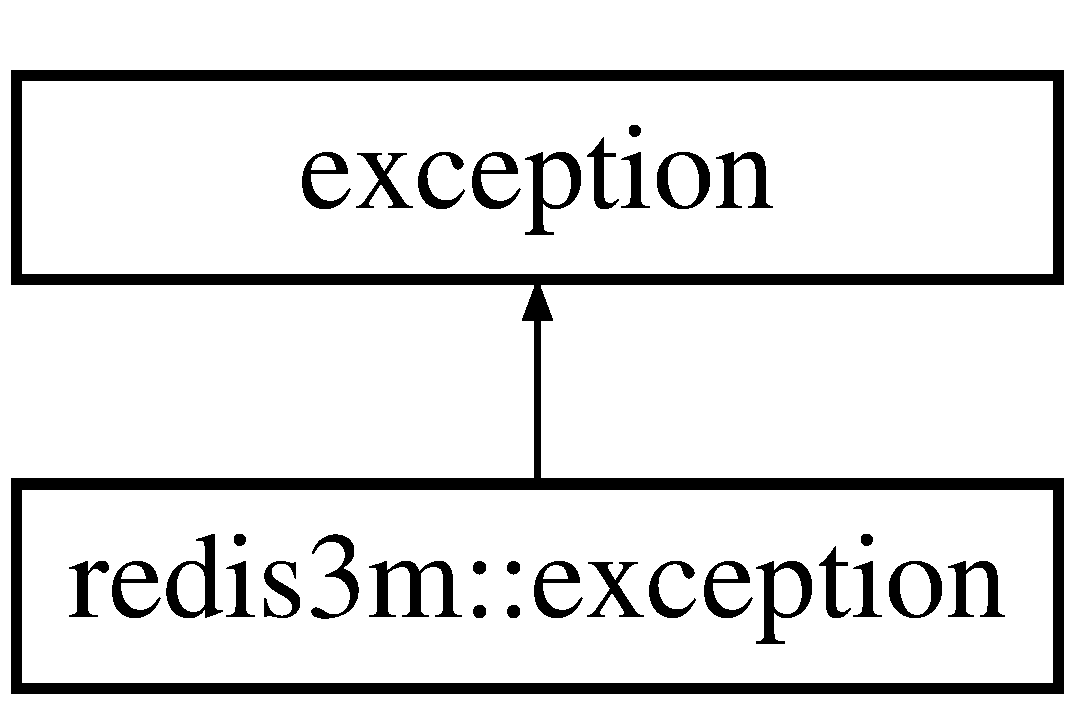
\includegraphics[height=2.000000cm]{classredis3m_1_1exception}
\end{center}
\end{figure}
\subsection*{Public Member Functions}
\begin{DoxyCompactItemize}
\item 
\hypertarget{classredis3m_1_1exception_a35b7fdb79d34ea259cf5a8473f20509c}{{\bfseries exception} (const std\-::string \&what)}\label{classredis3m_1_1exception_a35b7fdb79d34ea259cf5a8473f20509c}

\item 
\hypertarget{classredis3m_1_1exception_a08d93701a8d0d6900d2cae0304597f3c}{virtual const char $\ast$ {\bfseries what} ()}\label{classredis3m_1_1exception_a08d93701a8d0d6900d2cae0304597f3c}

\end{DoxyCompactItemize}


The documentation for this class was generated from the following file\-:\begin{DoxyCompactItemize}
\item 
include/redis3m/utils/exception.\-h\end{DoxyCompactItemize}

\hypertarget{classredis3m_1_1logging}{\section{redis3m\-:\-:logging Class Reference}
\label{classredis3m_1_1logging}\index{redis3m\-::logging@{redis3m\-::logging}}
}
\subsection*{Public Types}
\begin{DoxyCompactItemize}
\item 
\hypertarget{classredis3m_1_1logging_a155a3f862eb82e16a5af2decbf7237dd}{typedef boost\-::shared\-\_\-ptr\\*
$<$ \hyperlink{classredis3m_1_1logging}{logging} $>$ {\bfseries ptr\-\_\-t}}\label{classredis3m_1_1logging_a155a3f862eb82e16a5af2decbf7237dd}

\end{DoxyCompactItemize}
\subsection*{Public Member Functions}
\begin{DoxyCompactItemize}
\item 
\hypertarget{classredis3m_1_1logging_acca48cb20905358d5c137c56e49cfa8a}{virtual void {\bfseries debug\-\_\-impl} (const std\-::string \&s)}\label{classredis3m_1_1logging_acca48cb20905358d5c137c56e49cfa8a}

\item 
\hypertarget{classredis3m_1_1logging_a8cdb2eb07f644cf0abf298a525302be6}{virtual void {\bfseries error\-\_\-impl} (const std\-::string \&s)}\label{classredis3m_1_1logging_a8cdb2eb07f644cf0abf298a525302be6}

\end{DoxyCompactItemize}
\subsection*{Static Public Member Functions}
\begin{DoxyCompactItemize}
\item 
\hypertarget{classredis3m_1_1logging_a11dad7e613bad53fa01c0d199707944d}{static void {\bfseries debug} (const std\-::string \&s)}\label{classredis3m_1_1logging_a11dad7e613bad53fa01c0d199707944d}

\item 
\hypertarget{classredis3m_1_1logging_a4535e3c0f6299a8d8f233adc5ffa7651}{static void {\bfseries error} (const std\-::string \&s)}\label{classredis3m_1_1logging_a4535e3c0f6299a8d8f233adc5ffa7651}

\end{DoxyCompactItemize}


The documentation for this class was generated from the following files\-:\begin{DoxyCompactItemize}
\item 
include/redis3m/utils/logging.\-h\item 
src/utils/logging.\-cpp\end{DoxyCompactItemize}

\hypertarget{classredis3m_1_1patterns_1_1model}{\section{redis3m\-:\-:patterns\-:\-:model Class Reference}
\label{classredis3m_1_1patterns_1_1model}\index{redis3m\-::patterns\-::model@{redis3m\-::patterns\-::model}}
}


Class useful to define models used by \hyperlink{classredis3m_1_1patterns_1_1orm}{orm} and \hyperlink{classredis3m_1_1patterns_1_1simple__obj__store}{simple\-\_\-obj\-\_\-store}. R\-E\-D\-I\-S3\-M\-\_\-\-M\-O\-D\-E\-L\-\_\-\-R\-O\-\_\-\-A\-T\-T\-R\-I\-B\-U\-T\-E(type, name) macro defines automatically an attribute with a public getter. All fields need to be serialized to a std\-::map$<$std\-::string, std\-::string$>$. Model class contains various helpers to to that easily.  




{\ttfamily \#include $<$model.\-h$>$}

\subsection*{Public Member Functions}
\begin{DoxyCompactItemize}
\item 
\hypertarget{classredis3m_1_1patterns_1_1model_a844e576743580f8cb8edb5fd17426123}{\hyperlink{classredis3m_1_1patterns_1_1model_a844e576743580f8cb8edb5fd17426123}{model} ()}\label{classredis3m_1_1patterns_1_1model_a844e576743580f8cb8edb5fd17426123}

\begin{DoxyCompactList}\small\item\em Default constructor, use it to build a new object, still not saved to database. If you need to access data with getters, change \-\_\-loaded to true. Otherwise is better to leave it as false. \end{DoxyCompactList}\item 
\hyperlink{classredis3m_1_1patterns_1_1model_a68f1f52944af53408147818908ce5b96}{model} (const std\-::string \&\hyperlink{classredis3m_1_1patterns_1_1model_ac2b3983890b78356d9079a0cba78c5be}{id}, const std\-::map$<$ std\-::string, std\-::string $>$ \&map)
\begin{DoxyCompactList}\small\item\em Contructor called by orm or \hyperlink{classredis3m_1_1patterns_1_1simple__obj__store}{simple\-\_\-obj\-\_\-store} pattern. Used to fill object with data from database, call it from subclasses passing parameters as-\/is. It will set \-\_\-loaded to true, because data stored on this object is correct, as it's just retrieved from database. \end{DoxyCompactList}\item 
std\-::map$<$ std\-::string, \\*
std\-::string $>$ \hyperlink{classredis3m_1_1patterns_1_1model_ae5060af845197891c8f78240084e0463}{to\-\_\-map} ()
\begin{DoxyCompactList}\small\item\em Serialize all object data to a string\-:string map, it will be saved on Redis on a Hash. \end{DoxyCompactList}\item 
const std\-::string \& \hyperlink{classredis3m_1_1patterns_1_1model_ac2b3983890b78356d9079a0cba78c5be}{id} () const 
\begin{DoxyCompactList}\small\item\em Object unique identifier. \end{DoxyCompactList}\item 
bool \hyperlink{classredis3m_1_1patterns_1_1model_ac2ad745d637383d2cc42b6a1e15a82d6}{loaded} () const 
\begin{DoxyCompactList}\small\item\em If true means that object data is valid, as just get from database. \end{DoxyCompactList}\end{DoxyCompactItemize}
\subsection*{Static Public Member Functions}
\begin{DoxyCompactItemize}
\item 
static std\-::vector$<$ std\-::string $>$ \hyperlink{classredis3m_1_1patterns_1_1model_a250c0e67b38d5f2cc0f3dfd43ebc651e}{indices} ()
\begin{DoxyCompactList}\small\item\em A vector of fields to be indexed, used by Orm. \end{DoxyCompactList}\item 
static std\-::vector$<$ std\-::string $>$ \hyperlink{classredis3m_1_1patterns_1_1model_af8a02d965738e983649b27a6c87d34a6}{uniques} ()
\begin{DoxyCompactList}\small\item\em A vector of fields to be indexed in a unique fashion, used by Orm. \end{DoxyCompactList}\item 
static std\-::vector$<$ std\-::string $>$ \hyperlink{classredis3m_1_1patterns_1_1model_ad519cef941cae44d1a8da302558dd439}{tracked} ()
\begin{DoxyCompactList}\small\item\em Keys associated with a Model, may be sets or lists usually. They will be saved as $<$\-Modelname$>$\-:$<$modelid$>$\-:$<$keyname$>$ \end{DoxyCompactList}\end{DoxyCompactItemize}
\subsection*{Static Protected Member Functions}
\begin{DoxyCompactItemize}
\item 
static std\-::string \hyperlink{classredis3m_1_1patterns_1_1model_a10671593bb12a3c020e13903f72a457a}{read\-\_\-str\-\_\-from\-\_\-map} (const std\-::map$<$ std\-::string, std\-::string $>$ \&map, const std\-::string \&key, const std\-::string \&default\-\_\-value=\char`\"{}\char`\"{})
\begin{DoxyCompactList}\small\item\em Convenient method to get a field from a map, or returning a default value if the key is not present. Useful on constructor. \end{DoxyCompactList}\item 
static void \hyperlink{classredis3m_1_1patterns_1_1model_af81c69ba1d9b967af6f461fb672695db}{write\-\_\-str\-\_\-to\-\_\-map} (std\-::map$<$ std\-::string, std\-::string $>$ \&map, const std\-::string \&key, const std\-::string \&value, const std\-::string \&default\-\_\-value=\char`\"{}\char`\"{})
\begin{DoxyCompactList}\small\item\em Write a string to a map, useful on \hyperlink{classredis3m_1_1patterns_1_1model_ae5060af845197891c8f78240084e0463}{to\-\_\-map()} method. It saves value on the map only if it's different from default. \end{DoxyCompactList}\item 
{\footnotesize template$<$typename Integer\-Type $>$ }\\static Integer\-Type \hyperlink{classredis3m_1_1patterns_1_1model_a48f7240f426ef5904483ba9159b672e1}{read\-\_\-int\-\_\-from\-\_\-map} (const std\-::map$<$ std\-::string, std\-::string $>$ \&map, const std\-::string \&key, const Integer\-Type default\-\_\-value=0)
\begin{DoxyCompactList}\small\item\em Read an integer from map, otherwise use the specified default value (0) \end{DoxyCompactList}\item 
{\footnotesize template$<$typename Integer\-Type $>$ }\\static void \hyperlink{classredis3m_1_1patterns_1_1model_aee5174b2c37a0b7cd603a1b9dfc82ad2}{write\-\_\-int\-\_\-to\-\_\-map} (std\-::map$<$ std\-::string, std\-::string $>$ \&map, const std\-::string \&key, const Integer\-Type value, const Integer\-Type default\-\_\-value=0)
\begin{DoxyCompactList}\small\item\em Write an integer to a map, only if it's different from default value. \end{DoxyCompactList}\item 
static bool \hyperlink{classredis3m_1_1patterns_1_1model_a7923fa55c6eca5f1398e08be1c0b776f}{read\-\_\-bool\-\_\-from\-\_\-map} (const std\-::map$<$ std\-::string, std\-::string $>$ \&map, const std\-::string \&key)
\begin{DoxyCompactList}\small\item\em Read a boolean from a map. \end{DoxyCompactList}\item 
static void \hyperlink{classredis3m_1_1patterns_1_1model_a667ee0111f852a5f0594f51252319b6e}{write\-\_\-bool\-\_\-to\-\_\-map} (std\-::map$<$ std\-::string, std\-::string $>$ \&map, const std\-::string \&key, const bool value)
\begin{DoxyCompactList}\small\item\em Write a boolean to a map, only if it's true. \end{DoxyCompactList}\end{DoxyCompactItemize}
\subsection*{Protected Attributes}
\begin{DoxyCompactItemize}
\item 
\hypertarget{classredis3m_1_1patterns_1_1model_a1277b5e895e3b17ff03586455c8ed099}{std\-::string \hyperlink{classredis3m_1_1patterns_1_1model_a1277b5e895e3b17ff03586455c8ed099}{\-\_\-id}}\label{classredis3m_1_1patterns_1_1model_a1277b5e895e3b17ff03586455c8ed099}

\begin{DoxyCompactList}\small\item\em Unique identifier of the object, subclasses can set it to a custom value. \end{DoxyCompactList}\item 
\hypertarget{classredis3m_1_1patterns_1_1model_a724e4b494460ea475844e70b8bd2599b}{bool \hyperlink{classredis3m_1_1patterns_1_1model_a724e4b494460ea475844e70b8bd2599b}{\-\_\-loaded}}\label{classredis3m_1_1patterns_1_1model_a724e4b494460ea475844e70b8bd2599b}

\begin{DoxyCompactList}\small\item\em If this flag is true, data contained by an instance are correct, means that they reflect something stored on database. Can be set to true even for new object, still not saved, if it's necessary (by subclasses). \end{DoxyCompactList}\end{DoxyCompactItemize}


\subsection{Detailed Description}
Class useful to define models used by \hyperlink{classredis3m_1_1patterns_1_1orm}{orm} and \hyperlink{classredis3m_1_1patterns_1_1simple__obj__store}{simple\-\_\-obj\-\_\-store}. R\-E\-D\-I\-S3\-M\-\_\-\-M\-O\-D\-E\-L\-\_\-\-R\-O\-\_\-\-A\-T\-T\-R\-I\-B\-U\-T\-E(type, name) macro defines automatically an attribute with a public getter. All fields need to be serialized to a std\-::map$<$std\-::string, std\-::string$>$. Model class contains various helpers to to that easily. 

\subsection{Constructor \& Destructor Documentation}
\hypertarget{classredis3m_1_1patterns_1_1model_a68f1f52944af53408147818908ce5b96}{\index{redis3m\-::patterns\-::model@{redis3m\-::patterns\-::model}!model@{model}}
\index{model@{model}!redis3m::patterns::model@{redis3m\-::patterns\-::model}}
\subsubsection[{model}]{\setlength{\rightskip}{0pt plus 5cm}redis3m\-::patterns\-::model\-::model (
\begin{DoxyParamCaption}
\item[{const std\-::string \&}]{id, }
\item[{const std\-::map$<$ std\-::string, std\-::string $>$ \&}]{map}
\end{DoxyParamCaption}
)\hspace{0.3cm}{\ttfamily [inline]}}}\label{classredis3m_1_1patterns_1_1model_a68f1f52944af53408147818908ce5b96}


Contructor called by orm or \hyperlink{classredis3m_1_1patterns_1_1simple__obj__store}{simple\-\_\-obj\-\_\-store} pattern. Used to fill object with data from database, call it from subclasses passing parameters as-\/is. It will set \-\_\-loaded to true, because data stored on this object is correct, as it's just retrieved from database. 


\begin{DoxyParams}{Parameters}
{\em id} & identifier of object \\
\hline
{\em map} & serialized fields \\
\hline
\end{DoxyParams}


\subsection{Member Function Documentation}
\hypertarget{classredis3m_1_1patterns_1_1model_ac2b3983890b78356d9079a0cba78c5be}{\index{redis3m\-::patterns\-::model@{redis3m\-::patterns\-::model}!id@{id}}
\index{id@{id}!redis3m::patterns::model@{redis3m\-::patterns\-::model}}
\subsubsection[{id}]{\setlength{\rightskip}{0pt plus 5cm}const std\-::string\& redis3m\-::patterns\-::model\-::id (
\begin{DoxyParamCaption}
{}
\end{DoxyParamCaption}
) const\hspace{0.3cm}{\ttfamily [inline]}}}\label{classredis3m_1_1patterns_1_1model_ac2b3983890b78356d9079a0cba78c5be}


Object unique identifier. 

\begin{DoxyReturn}{Returns}

\end{DoxyReturn}
\hypertarget{classredis3m_1_1patterns_1_1model_a250c0e67b38d5f2cc0f3dfd43ebc651e}{\index{redis3m\-::patterns\-::model@{redis3m\-::patterns\-::model}!indices@{indices}}
\index{indices@{indices}!redis3m::patterns::model@{redis3m\-::patterns\-::model}}
\subsubsection[{indices}]{\setlength{\rightskip}{0pt plus 5cm}static std\-::vector$<$ std\-::string $>$ redis3m\-::patterns\-::model\-::indices (
\begin{DoxyParamCaption}
{}
\end{DoxyParamCaption}
)\hspace{0.3cm}{\ttfamily [inline]}, {\ttfamily [static]}}}\label{classredis3m_1_1patterns_1_1model_a250c0e67b38d5f2cc0f3dfd43ebc651e}


A vector of fields to be indexed, used by Orm. 

\begin{DoxyReturn}{Returns}

\end{DoxyReturn}
\hypertarget{classredis3m_1_1patterns_1_1model_ac2ad745d637383d2cc42b6a1e15a82d6}{\index{redis3m\-::patterns\-::model@{redis3m\-::patterns\-::model}!loaded@{loaded}}
\index{loaded@{loaded}!redis3m::patterns::model@{redis3m\-::patterns\-::model}}
\subsubsection[{loaded}]{\setlength{\rightskip}{0pt plus 5cm}bool redis3m\-::patterns\-::model\-::loaded (
\begin{DoxyParamCaption}
{}
\end{DoxyParamCaption}
) const\hspace{0.3cm}{\ttfamily [inline]}}}\label{classredis3m_1_1patterns_1_1model_ac2ad745d637383d2cc42b6a1e15a82d6}


If true means that object data is valid, as just get from database. 

\begin{DoxyReturn}{Returns}

\end{DoxyReturn}
\hypertarget{classredis3m_1_1patterns_1_1model_a7923fa55c6eca5f1398e08be1c0b776f}{\index{redis3m\-::patterns\-::model@{redis3m\-::patterns\-::model}!read\-\_\-bool\-\_\-from\-\_\-map@{read\-\_\-bool\-\_\-from\-\_\-map}}
\index{read\-\_\-bool\-\_\-from\-\_\-map@{read\-\_\-bool\-\_\-from\-\_\-map}!redis3m::patterns::model@{redis3m\-::patterns\-::model}}
\subsubsection[{read\-\_\-bool\-\_\-from\-\_\-map}]{\setlength{\rightskip}{0pt plus 5cm}static bool redis3m\-::patterns\-::model\-::read\-\_\-bool\-\_\-from\-\_\-map (
\begin{DoxyParamCaption}
\item[{const std\-::map$<$ std\-::string, std\-::string $>$ \&}]{map, }
\item[{const std\-::string \&}]{key}
\end{DoxyParamCaption}
)\hspace{0.3cm}{\ttfamily [inline]}, {\ttfamily [static]}, {\ttfamily [protected]}}}\label{classredis3m_1_1patterns_1_1model_a7923fa55c6eca5f1398e08be1c0b776f}


Read a boolean from a map. 


\begin{DoxyParams}{Parameters}
{\em map} & \\
\hline
{\em key} & \\
\hline
\end{DoxyParams}
\begin{DoxyReturn}{Returns}

\end{DoxyReturn}
\hypertarget{classredis3m_1_1patterns_1_1model_a48f7240f426ef5904483ba9159b672e1}{\index{redis3m\-::patterns\-::model@{redis3m\-::patterns\-::model}!read\-\_\-int\-\_\-from\-\_\-map@{read\-\_\-int\-\_\-from\-\_\-map}}
\index{read\-\_\-int\-\_\-from\-\_\-map@{read\-\_\-int\-\_\-from\-\_\-map}!redis3m::patterns::model@{redis3m\-::patterns\-::model}}
\subsubsection[{read\-\_\-int\-\_\-from\-\_\-map}]{\setlength{\rightskip}{0pt plus 5cm}template$<$typename Integer\-Type $>$ static Integer\-Type redis3m\-::patterns\-::model\-::read\-\_\-int\-\_\-from\-\_\-map (
\begin{DoxyParamCaption}
\item[{const std\-::map$<$ std\-::string, std\-::string $>$ \&}]{map, }
\item[{const std\-::string \&}]{key, }
\item[{const Integer\-Type}]{default\-\_\-value = {\ttfamily 0}}
\end{DoxyParamCaption}
)\hspace{0.3cm}{\ttfamily [inline]}, {\ttfamily [static]}, {\ttfamily [protected]}}}\label{classredis3m_1_1patterns_1_1model_a48f7240f426ef5904483ba9159b672e1}


Read an integer from map, otherwise use the specified default value (0) 


\begin{DoxyParams}{Parameters}
{\em map} & \\
\hline
{\em key} & \\
\hline
{\em default\-\_\-value} & \\
\hline
\end{DoxyParams}
\begin{DoxyReturn}{Returns}

\end{DoxyReturn}
\hypertarget{classredis3m_1_1patterns_1_1model_a10671593bb12a3c020e13903f72a457a}{\index{redis3m\-::patterns\-::model@{redis3m\-::patterns\-::model}!read\-\_\-str\-\_\-from\-\_\-map@{read\-\_\-str\-\_\-from\-\_\-map}}
\index{read\-\_\-str\-\_\-from\-\_\-map@{read\-\_\-str\-\_\-from\-\_\-map}!redis3m::patterns::model@{redis3m\-::patterns\-::model}}
\subsubsection[{read\-\_\-str\-\_\-from\-\_\-map}]{\setlength{\rightskip}{0pt plus 5cm}static std\-::string redis3m\-::patterns\-::model\-::read\-\_\-str\-\_\-from\-\_\-map (
\begin{DoxyParamCaption}
\item[{const std\-::map$<$ std\-::string, std\-::string $>$ \&}]{map, }
\item[{const std\-::string \&}]{key, }
\item[{const std\-::string \&}]{default\-\_\-value = {\ttfamily \char`\"{}\char`\"{}}}
\end{DoxyParamCaption}
)\hspace{0.3cm}{\ttfamily [inline]}, {\ttfamily [static]}, {\ttfamily [protected]}}}\label{classredis3m_1_1patterns_1_1model_a10671593bb12a3c020e13903f72a457a}


Convenient method to get a field from a map, or returning a default value if the key is not present. Useful on constructor. 


\begin{DoxyParams}{Parameters}
{\em map} & \\
\hline
{\em key} & \\
\hline
{\em default\-\_\-value} & \\
\hline
\end{DoxyParams}
\begin{DoxyReturn}{Returns}

\end{DoxyReturn}
\hypertarget{classredis3m_1_1patterns_1_1model_ae5060af845197891c8f78240084e0463}{\index{redis3m\-::patterns\-::model@{redis3m\-::patterns\-::model}!to\-\_\-map@{to\-\_\-map}}
\index{to\-\_\-map@{to\-\_\-map}!redis3m::patterns::model@{redis3m\-::patterns\-::model}}
\subsubsection[{to\-\_\-map}]{\setlength{\rightskip}{0pt plus 5cm}std\-::map$<$std\-::string, std\-::string$>$ redis3m\-::patterns\-::model\-::to\-\_\-map (
\begin{DoxyParamCaption}
{}
\end{DoxyParamCaption}
)\hspace{0.3cm}{\ttfamily [inline]}}}\label{classredis3m_1_1patterns_1_1model_ae5060af845197891c8f78240084e0463}


Serialize all object data to a string\-:string map, it will be saved on Redis on a Hash. 

\begin{DoxyReturn}{Returns}

\end{DoxyReturn}
\hypertarget{classredis3m_1_1patterns_1_1model_ad519cef941cae44d1a8da302558dd439}{\index{redis3m\-::patterns\-::model@{redis3m\-::patterns\-::model}!tracked@{tracked}}
\index{tracked@{tracked}!redis3m::patterns::model@{redis3m\-::patterns\-::model}}
\subsubsection[{tracked}]{\setlength{\rightskip}{0pt plus 5cm}static std\-::vector$<$std\-::string$>$ redis3m\-::patterns\-::model\-::tracked (
\begin{DoxyParamCaption}
{}
\end{DoxyParamCaption}
)\hspace{0.3cm}{\ttfamily [inline]}, {\ttfamily [static]}}}\label{classredis3m_1_1patterns_1_1model_ad519cef941cae44d1a8da302558dd439}


Keys associated with a Model, may be sets or lists usually. They will be saved as $<$\-Modelname$>$\-:$<$modelid$>$\-:$<$keyname$>$ 

\begin{DoxyReturn}{Returns}
A vector of keys, 
\end{DoxyReturn}
\hypertarget{classredis3m_1_1patterns_1_1model_af8a02d965738e983649b27a6c87d34a6}{\index{redis3m\-::patterns\-::model@{redis3m\-::patterns\-::model}!uniques@{uniques}}
\index{uniques@{uniques}!redis3m::patterns::model@{redis3m\-::patterns\-::model}}
\subsubsection[{uniques}]{\setlength{\rightskip}{0pt plus 5cm}static std\-::vector$<$ std\-::string $>$ redis3m\-::patterns\-::model\-::uniques (
\begin{DoxyParamCaption}
{}
\end{DoxyParamCaption}
)\hspace{0.3cm}{\ttfamily [inline]}, {\ttfamily [static]}}}\label{classredis3m_1_1patterns_1_1model_af8a02d965738e983649b27a6c87d34a6}


A vector of fields to be indexed in a unique fashion, used by Orm. 

\begin{DoxyReturn}{Returns}

\end{DoxyReturn}
\hypertarget{classredis3m_1_1patterns_1_1model_a667ee0111f852a5f0594f51252319b6e}{\index{redis3m\-::patterns\-::model@{redis3m\-::patterns\-::model}!write\-\_\-bool\-\_\-to\-\_\-map@{write\-\_\-bool\-\_\-to\-\_\-map}}
\index{write\-\_\-bool\-\_\-to\-\_\-map@{write\-\_\-bool\-\_\-to\-\_\-map}!redis3m::patterns::model@{redis3m\-::patterns\-::model}}
\subsubsection[{write\-\_\-bool\-\_\-to\-\_\-map}]{\setlength{\rightskip}{0pt plus 5cm}static void redis3m\-::patterns\-::model\-::write\-\_\-bool\-\_\-to\-\_\-map (
\begin{DoxyParamCaption}
\item[{std\-::map$<$ std\-::string, std\-::string $>$ \&}]{map, }
\item[{const std\-::string \&}]{key, }
\item[{const bool}]{value}
\end{DoxyParamCaption}
)\hspace{0.3cm}{\ttfamily [inline]}, {\ttfamily [static]}, {\ttfamily [protected]}}}\label{classredis3m_1_1patterns_1_1model_a667ee0111f852a5f0594f51252319b6e}


Write a boolean to a map, only if it's true. 


\begin{DoxyParams}{Parameters}
{\em map} & \\
\hline
{\em key} & \\
\hline
{\em value} & \\
\hline
\end{DoxyParams}
\hypertarget{classredis3m_1_1patterns_1_1model_aee5174b2c37a0b7cd603a1b9dfc82ad2}{\index{redis3m\-::patterns\-::model@{redis3m\-::patterns\-::model}!write\-\_\-int\-\_\-to\-\_\-map@{write\-\_\-int\-\_\-to\-\_\-map}}
\index{write\-\_\-int\-\_\-to\-\_\-map@{write\-\_\-int\-\_\-to\-\_\-map}!redis3m::patterns::model@{redis3m\-::patterns\-::model}}
\subsubsection[{write\-\_\-int\-\_\-to\-\_\-map}]{\setlength{\rightskip}{0pt plus 5cm}template$<$typename Integer\-Type $>$ static void redis3m\-::patterns\-::model\-::write\-\_\-int\-\_\-to\-\_\-map (
\begin{DoxyParamCaption}
\item[{std\-::map$<$ std\-::string, std\-::string $>$ \&}]{map, }
\item[{const std\-::string \&}]{key, }
\item[{const Integer\-Type}]{value, }
\item[{const Integer\-Type}]{default\-\_\-value = {\ttfamily 0}}
\end{DoxyParamCaption}
)\hspace{0.3cm}{\ttfamily [inline]}, {\ttfamily [static]}, {\ttfamily [protected]}}}\label{classredis3m_1_1patterns_1_1model_aee5174b2c37a0b7cd603a1b9dfc82ad2}


Write an integer to a map, only if it's different from default value. 


\begin{DoxyParams}{Parameters}
{\em map} & \\
\hline
{\em key} & \\
\hline
{\em value} & \\
\hline
{\em default\-\_\-value} & \\
\hline
\end{DoxyParams}
\hypertarget{classredis3m_1_1patterns_1_1model_af81c69ba1d9b967af6f461fb672695db}{\index{redis3m\-::patterns\-::model@{redis3m\-::patterns\-::model}!write\-\_\-str\-\_\-to\-\_\-map@{write\-\_\-str\-\_\-to\-\_\-map}}
\index{write\-\_\-str\-\_\-to\-\_\-map@{write\-\_\-str\-\_\-to\-\_\-map}!redis3m::patterns::model@{redis3m\-::patterns\-::model}}
\subsubsection[{write\-\_\-str\-\_\-to\-\_\-map}]{\setlength{\rightskip}{0pt plus 5cm}static void redis3m\-::patterns\-::model\-::write\-\_\-str\-\_\-to\-\_\-map (
\begin{DoxyParamCaption}
\item[{std\-::map$<$ std\-::string, std\-::string $>$ \&}]{map, }
\item[{const std\-::string \&}]{key, }
\item[{const std\-::string \&}]{value, }
\item[{const std\-::string \&}]{default\-\_\-value = {\ttfamily \char`\"{}\char`\"{}}}
\end{DoxyParamCaption}
)\hspace{0.3cm}{\ttfamily [inline]}, {\ttfamily [static]}, {\ttfamily [protected]}}}\label{classredis3m_1_1patterns_1_1model_af81c69ba1d9b967af6f461fb672695db}


Write a string to a map, useful on \hyperlink{classredis3m_1_1patterns_1_1model_ae5060af845197891c8f78240084e0463}{to\-\_\-map()} method. It saves value on the map only if it's different from default. 


\begin{DoxyParams}{Parameters}
{\em map} & \\
\hline
{\em key} & \\
\hline
{\em value} & \\
\hline
{\em default\-\_\-value} & \\
\hline
\end{DoxyParams}


The documentation for this class was generated from the following file\-:\begin{DoxyCompactItemize}
\item 
include/redis3m/patterns/model.\-h\end{DoxyCompactItemize}

\hypertarget{classredis3m_1_1patterns_1_1orm}{\section{redis3m\-:\-:patterns\-:\-:orm$<$ Model $>$ Class Template Reference}
\label{classredis3m_1_1patterns_1_1orm}\index{redis3m\-::patterns\-::orm$<$ Model $>$@{redis3m\-::patterns\-::orm$<$ Model $>$}}
}


Object-\/\-Redis-\/\-Mapper is a convenient pattern to store object on Redis. Useful when you need classic C\-R\-U\-D operations. It's compatible and inspired by \href{http://github.com/soveran/ohm}{\tt http\-://github.\-com/soveran/ohm}. Data can be indexed and it supports also uniques. To use it make a subclass of \hyperlink{classredis3m_1_1patterns_1_1model}{model} to model your attribute and use it to fill orm template parameter.  




{\ttfamily \#include $<$orm.\-h$>$}

\subsection*{Public Member Functions}
\begin{DoxyCompactItemize}
\item 
Model \hyperlink{classredis3m_1_1patterns_1_1orm_a3e96c9961e2445ff7d399f7c4c131d90}{find\-\_\-by\-\_\-id} (connection\-::ptr\-\_\-t conn, const std\-::string \&id)
\begin{DoxyCompactList}\small\item\em As the name says, get an object from id specifying it's unique identifier. \end{DoxyCompactList}\item 
Model \hyperlink{classredis3m_1_1patterns_1_1orm_a8e3ef3bbd7a44779425c0cd603e8ffc5}{find\-\_\-by\-\_\-unique\-\_\-field} (connection\-::ptr\-\_\-t conn, const std\-::string \&field, const std\-::string \&value)
\begin{DoxyCompactList}\small\item\em Find an object by using a unique field. \end{DoxyCompactList}\item 
bool \hyperlink{classredis3m_1_1patterns_1_1orm_a68ed176f8848c5c30612a8d29fb341d6}{exists\-\_\-by\-\_\-id} (connection\-::ptr\-\_\-t conn, const std\-::string \&id)
\begin{DoxyCompactList}\small\item\em Check if an object exists or not. \end{DoxyCompactList}\item 
std\-::string \hyperlink{classredis3m_1_1patterns_1_1orm_ae9618fa5fc90c05ad75dab2bd8979a66}{save} (connection\-::ptr\-\_\-t conn, const Model \&\hyperlink{classredis3m_1_1patterns_1_1model}{model})
\begin{DoxyCompactList}\small\item\em Save an object on database, or update it if it's already present. \end{DoxyCompactList}\item 
void \hyperlink{classredis3m_1_1patterns_1_1orm_a821adbf0bafae4563104977c7982882a}{remove} (connection\-::ptr\-\_\-t conn, const Model \&\hyperlink{classredis3m_1_1patterns_1_1model}{model})
\begin{DoxyCompactList}\small\item\em Remove object and all related data from database. \end{DoxyCompactList}\item 
\hypertarget{classredis3m_1_1patterns_1_1orm_aa8b6e4d42bef93974070001ec4c5ab60}{std\-::vector$<$ std\-::string $>$ {\bfseries list\-\_\-members} (connection\-::ptr\-\_\-t conn, const Model \&m, const std\-::string \&list\-\_\-name)}\label{classredis3m_1_1patterns_1_1orm_aa8b6e4d42bef93974070001ec4c5ab60}

\item 
\hypertarget{classredis3m_1_1patterns_1_1orm_a790d4963363d3f7af3a27f3c92261d6e}{void {\bfseries set\-\_\-add} (connection\-::ptr\-\_\-t conn, const Model \&m, const std\-::string \&set\-\_\-name, const std\-::string \&entry)}\label{classredis3m_1_1patterns_1_1orm_a790d4963363d3f7af3a27f3c92261d6e}

\item 
\hypertarget{classredis3m_1_1patterns_1_1orm_a5e552563226e067d04defdfb0ed77f57}{void {\bfseries set\-\_\-remove} (connection\-::ptr\-\_\-t conn, const Model \&m, const std\-::string \&set\-\_\-name, const std\-::string \&entry)}\label{classredis3m_1_1patterns_1_1orm_a5e552563226e067d04defdfb0ed77f57}

\item 
\hypertarget{classredis3m_1_1patterns_1_1orm_ab6fb72124e1ea7550eb0b908b95ab86f}{std\-::set$<$ std\-::string $>$ {\bfseries set\-\_\-members} (connection\-::ptr\-\_\-t conn, const Model \&m, const std\-::string \&set\-\_\-name)}\label{classredis3m_1_1patterns_1_1orm_ab6fb72124e1ea7550eb0b908b95ab86f}

\item 
std\-::string \hyperlink{classredis3m_1_1patterns_1_1orm_a520433866ecfba1b4679d04af46603f3}{collection\-\_\-key} ()
\begin{DoxyCompactList}\small\item\em Redis key of a S\-E\-T containing all object ids. Useful for custom operations. Pay attention to mantain compatibility with all other functions. \end{DoxyCompactList}\item 
std\-::string \hyperlink{classredis3m_1_1patterns_1_1orm_a75199bb02a7e188a9cf60fdbbc4ec0be}{collection\-\_\-id\-\_\-key} ()
\begin{DoxyCompactList}\small\item\em Key containing an incremental counter, used to generate an id for new objects. Useful for custom operations. Pay attention to mantain compatibility with all other functions. \end{DoxyCompactList}\item 
std\-::string \hyperlink{classredis3m_1_1patterns_1_1orm_ad4232c86962fdb91a206fa3f78dabaa6}{model\-\_\-key} (const std\-::string \&id)
\begin{DoxyCompactList}\small\item\em Returns Redis Key used to save object data. \end{DoxyCompactList}\item 
std\-::string \hyperlink{classredis3m_1_1patterns_1_1orm_ad1b2ed504968d06a941588374c92b0ba}{tracked\-\_\-key} (const std\-::string \&id, const std\-::string \&key)
\begin{DoxyCompactList}\small\item\em Returns full key, related to object. \end{DoxyCompactList}\item 
\hypertarget{classredis3m_1_1patterns_1_1orm_ab18df7a4c6412ea15fd79d8b686a3757}{std\-::string {\bfseries indexed\-\_\-field\-\_\-key} (const std\-::string \&field, const std\-::string \&value)}\label{classredis3m_1_1patterns_1_1orm_ab18df7a4c6412ea15fd79d8b686a3757}

\item 
\hypertarget{classredis3m_1_1patterns_1_1orm_a4bf7085f7752f334e8070b3ca3f44ebf}{std\-::string {\bfseries unique\-\_\-field\-\_\-key} (const std\-::string \&field)}\label{classredis3m_1_1patterns_1_1orm_a4bf7085f7752f334e8070b3ca3f44ebf}

\end{DoxyCompactItemize}


\subsection{Detailed Description}
\subsubsection*{template$<$typename Model$>$class redis3m\-::patterns\-::orm$<$ Model $>$}

Object-\/\-Redis-\/\-Mapper is a convenient pattern to store object on Redis. Useful when you need classic C\-R\-U\-D operations. It's compatible and inspired by \href{http://github.com/soveran/ohm}{\tt http\-://github.\-com/soveran/ohm}. Data can be indexed and it supports also uniques. To use it make a subclass of \hyperlink{classredis3m_1_1patterns_1_1model}{model} to model your attribute and use it to fill orm template parameter. 

\subsection{Member Function Documentation}
\hypertarget{classredis3m_1_1patterns_1_1orm_a75199bb02a7e188a9cf60fdbbc4ec0be}{\index{redis3m\-::patterns\-::orm@{redis3m\-::patterns\-::orm}!collection\-\_\-id\-\_\-key@{collection\-\_\-id\-\_\-key}}
\index{collection\-\_\-id\-\_\-key@{collection\-\_\-id\-\_\-key}!redis3m::patterns::orm@{redis3m\-::patterns\-::orm}}
\subsubsection[{collection\-\_\-id\-\_\-key}]{\setlength{\rightskip}{0pt plus 5cm}template$<$typename Model $>$ std\-::string {\bf redis3m\-::patterns\-::orm}$<$ Model $>$\-::collection\-\_\-id\-\_\-key (
\begin{DoxyParamCaption}
{}
\end{DoxyParamCaption}
)\hspace{0.3cm}{\ttfamily [inline]}}}\label{classredis3m_1_1patterns_1_1orm_a75199bb02a7e188a9cf60fdbbc4ec0be}


Key containing an incremental counter, used to generate an id for new objects. Useful for custom operations. Pay attention to mantain compatibility with all other functions. 

\begin{DoxyReturn}{Returns}

\end{DoxyReturn}
\hypertarget{classredis3m_1_1patterns_1_1orm_a520433866ecfba1b4679d04af46603f3}{\index{redis3m\-::patterns\-::orm@{redis3m\-::patterns\-::orm}!collection\-\_\-key@{collection\-\_\-key}}
\index{collection\-\_\-key@{collection\-\_\-key}!redis3m::patterns::orm@{redis3m\-::patterns\-::orm}}
\subsubsection[{collection\-\_\-key}]{\setlength{\rightskip}{0pt plus 5cm}template$<$typename Model $>$ std\-::string {\bf redis3m\-::patterns\-::orm}$<$ Model $>$\-::collection\-\_\-key (
\begin{DoxyParamCaption}
{}
\end{DoxyParamCaption}
)\hspace{0.3cm}{\ttfamily [inline]}}}\label{classredis3m_1_1patterns_1_1orm_a520433866ecfba1b4679d04af46603f3}


Redis key of a S\-E\-T containing all object ids. Useful for custom operations. Pay attention to mantain compatibility with all other functions. 

\begin{DoxyReturn}{Returns}

\end{DoxyReturn}
\hypertarget{classredis3m_1_1patterns_1_1orm_a68ed176f8848c5c30612a8d29fb341d6}{\index{redis3m\-::patterns\-::orm@{redis3m\-::patterns\-::orm}!exists\-\_\-by\-\_\-id@{exists\-\_\-by\-\_\-id}}
\index{exists\-\_\-by\-\_\-id@{exists\-\_\-by\-\_\-id}!redis3m::patterns::orm@{redis3m\-::patterns\-::orm}}
\subsubsection[{exists\-\_\-by\-\_\-id}]{\setlength{\rightskip}{0pt plus 5cm}template$<$typename Model $>$ bool {\bf redis3m\-::patterns\-::orm}$<$ Model $>$\-::exists\-\_\-by\-\_\-id (
\begin{DoxyParamCaption}
\item[{connection\-::ptr\-\_\-t}]{conn, }
\item[{const std\-::string \&}]{id}
\end{DoxyParamCaption}
)\hspace{0.3cm}{\ttfamily [inline]}}}\label{classredis3m_1_1patterns_1_1orm_a68ed176f8848c5c30612a8d29fb341d6}


Check if an object exists or not. 


\begin{DoxyParams}{Parameters}
{\em conn} & \\
\hline
{\em id} & Unique identifier \\
\hline
\end{DoxyParams}
\begin{DoxyReturn}{Returns}

\end{DoxyReturn}
\hypertarget{classredis3m_1_1patterns_1_1orm_a3e96c9961e2445ff7d399f7c4c131d90}{\index{redis3m\-::patterns\-::orm@{redis3m\-::patterns\-::orm}!find\-\_\-by\-\_\-id@{find\-\_\-by\-\_\-id}}
\index{find\-\_\-by\-\_\-id@{find\-\_\-by\-\_\-id}!redis3m::patterns::orm@{redis3m\-::patterns\-::orm}}
\subsubsection[{find\-\_\-by\-\_\-id}]{\setlength{\rightskip}{0pt plus 5cm}template$<$typename Model $>$ Model {\bf redis3m\-::patterns\-::orm}$<$ Model $>$\-::find\-\_\-by\-\_\-id (
\begin{DoxyParamCaption}
\item[{connection\-::ptr\-\_\-t}]{conn, }
\item[{const std\-::string \&}]{id}
\end{DoxyParamCaption}
)\hspace{0.3cm}{\ttfamily [inline]}}}\label{classredis3m_1_1patterns_1_1orm_a3e96c9961e2445ff7d399f7c4c131d90}


As the name says, get an object from id specifying it's unique identifier. 


\begin{DoxyParams}{Parameters}
{\em conn} & \\
\hline
{\em id} & \\
\hline
\end{DoxyParams}
\begin{DoxyReturn}{Returns}
Use \hyperlink{classredis3m_1_1patterns_1_1model_ac2ad745d637383d2cc42b6a1e15a82d6}{model.\-loaded()} to check if it's valid or not 
\end{DoxyReturn}
\hypertarget{classredis3m_1_1patterns_1_1orm_a8e3ef3bbd7a44779425c0cd603e8ffc5}{\index{redis3m\-::patterns\-::orm@{redis3m\-::patterns\-::orm}!find\-\_\-by\-\_\-unique\-\_\-field@{find\-\_\-by\-\_\-unique\-\_\-field}}
\index{find\-\_\-by\-\_\-unique\-\_\-field@{find\-\_\-by\-\_\-unique\-\_\-field}!redis3m::patterns::orm@{redis3m\-::patterns\-::orm}}
\subsubsection[{find\-\_\-by\-\_\-unique\-\_\-field}]{\setlength{\rightskip}{0pt plus 5cm}template$<$typename Model $>$ Model {\bf redis3m\-::patterns\-::orm}$<$ Model $>$\-::find\-\_\-by\-\_\-unique\-\_\-field (
\begin{DoxyParamCaption}
\item[{connection\-::ptr\-\_\-t}]{conn, }
\item[{const std\-::string \&}]{field, }
\item[{const std\-::string \&}]{value}
\end{DoxyParamCaption}
)\hspace{0.3cm}{\ttfamily [inline]}}}\label{classredis3m_1_1patterns_1_1orm_a8e3ef3bbd7a44779425c0cd603e8ffc5}


Find an object by using a unique field. 


\begin{DoxyParams}{Parameters}
{\em conn} & \\
\hline
{\em field} & name of field, should be returned by \hyperlink{classredis3m_1_1patterns_1_1model_af8a02d965738e983649b27a6c87d34a6}{model\-::uniques} \\
\hline
{\em value} & \\
\hline
\end{DoxyParams}
\begin{DoxyReturn}{Returns}
Use \hyperlink{classredis3m_1_1patterns_1_1model_ac2ad745d637383d2cc42b6a1e15a82d6}{model.\-loaded()} to check if it's valid or not 
\end{DoxyReturn}
\hypertarget{classredis3m_1_1patterns_1_1orm_ad4232c86962fdb91a206fa3f78dabaa6}{\index{redis3m\-::patterns\-::orm@{redis3m\-::patterns\-::orm}!model\-\_\-key@{model\-\_\-key}}
\index{model\-\_\-key@{model\-\_\-key}!redis3m::patterns::orm@{redis3m\-::patterns\-::orm}}
\subsubsection[{model\-\_\-key}]{\setlength{\rightskip}{0pt plus 5cm}template$<$typename Model $>$ std\-::string {\bf redis3m\-::patterns\-::orm}$<$ Model $>$\-::model\-\_\-key (
\begin{DoxyParamCaption}
\item[{const std\-::string \&}]{id}
\end{DoxyParamCaption}
)\hspace{0.3cm}{\ttfamily [inline]}}}\label{classredis3m_1_1patterns_1_1orm_ad4232c86962fdb91a206fa3f78dabaa6}


Returns Redis Key used to save object data. 


\begin{DoxyParams}{Parameters}
{\em id} & \\
\hline
\end{DoxyParams}
\begin{DoxyReturn}{Returns}

\end{DoxyReturn}
\hypertarget{classredis3m_1_1patterns_1_1orm_a821adbf0bafae4563104977c7982882a}{\index{redis3m\-::patterns\-::orm@{redis3m\-::patterns\-::orm}!remove@{remove}}
\index{remove@{remove}!redis3m::patterns::orm@{redis3m\-::patterns\-::orm}}
\subsubsection[{remove}]{\setlength{\rightskip}{0pt plus 5cm}template$<$typename Model $>$ void {\bf redis3m\-::patterns\-::orm}$<$ Model $>$\-::remove (
\begin{DoxyParamCaption}
\item[{connection\-::ptr\-\_\-t}]{conn, }
\item[{const Model \&}]{model}
\end{DoxyParamCaption}
)\hspace{0.3cm}{\ttfamily [inline]}}}\label{classredis3m_1_1patterns_1_1orm_a821adbf0bafae4563104977c7982882a}


Remove object and all related data from database. 


\begin{DoxyParams}{Parameters}
{\em conn} & \\
\hline
{\em model} & \\
\hline
\end{DoxyParams}
\hypertarget{classredis3m_1_1patterns_1_1orm_ae9618fa5fc90c05ad75dab2bd8979a66}{\index{redis3m\-::patterns\-::orm@{redis3m\-::patterns\-::orm}!save@{save}}
\index{save@{save}!redis3m::patterns::orm@{redis3m\-::patterns\-::orm}}
\subsubsection[{save}]{\setlength{\rightskip}{0pt plus 5cm}template$<$typename Model $>$ std\-::string {\bf redis3m\-::patterns\-::orm}$<$ Model $>$\-::save (
\begin{DoxyParamCaption}
\item[{connection\-::ptr\-\_\-t}]{conn, }
\item[{const Model \&}]{model}
\end{DoxyParamCaption}
)\hspace{0.3cm}{\ttfamily [inline]}}}\label{classredis3m_1_1patterns_1_1orm_ae9618fa5fc90c05ad75dab2bd8979a66}


Save an object on database, or update it if it's already present. 


\begin{DoxyParams}{Parameters}
{\em conn} & \\
\hline
{\em model} & \\
\hline
\end{DoxyParams}
\begin{DoxyReturn}{Returns}
unique identifier of the object, a new one on creation. 
\end{DoxyReturn}
\hypertarget{classredis3m_1_1patterns_1_1orm_ad1b2ed504968d06a941588374c92b0ba}{\index{redis3m\-::patterns\-::orm@{redis3m\-::patterns\-::orm}!tracked\-\_\-key@{tracked\-\_\-key}}
\index{tracked\-\_\-key@{tracked\-\_\-key}!redis3m::patterns::orm@{redis3m\-::patterns\-::orm}}
\subsubsection[{tracked\-\_\-key}]{\setlength{\rightskip}{0pt plus 5cm}template$<$typename Model $>$ std\-::string {\bf redis3m\-::patterns\-::orm}$<$ Model $>$\-::tracked\-\_\-key (
\begin{DoxyParamCaption}
\item[{const std\-::string \&}]{id, }
\item[{const std\-::string \&}]{key}
\end{DoxyParamCaption}
)\hspace{0.3cm}{\ttfamily [inline]}}}\label{classredis3m_1_1patterns_1_1orm_ad1b2ed504968d06a941588374c92b0ba}


Returns full key, related to object. 


\begin{DoxyParams}{Parameters}
{\em id} & \\
\hline
{\em key} & \\
\hline
\end{DoxyParams}
\begin{DoxyReturn}{Returns}

\end{DoxyReturn}


The documentation for this class was generated from the following file\-:\begin{DoxyCompactItemize}
\item 
include/redis3m/patterns/orm.\-h\end{DoxyCompactItemize}

\hypertarget{classredis3m_1_1reply}{\section{redis3m\-:\-:reply Class Reference}
\label{classredis3m_1_1reply}\index{redis3m\-::reply@{redis3m\-::reply}}
}


Represent a reply received from redis server.  




{\ttfamily \#include $<$reply.\-h$>$}

\subsection*{Public Types}
\begin{DoxyCompactItemize}
\item 
enum \hyperlink{classredis3m_1_1reply_ac44942a4ec175e767ce119d452ffafd6}{type\-\_\-t} \{ \\*
{\bfseries S\-T\-R\-I\-N\-G} = 1, 
{\bfseries A\-R\-R\-A\-Y} = 2, 
{\bfseries I\-N\-T\-E\-G\-E\-R} = 3, 
{\bfseries N\-I\-L} = 4, 
\\*
{\bfseries S\-T\-A\-T\-U\-S} = 5, 
{\bfseries E\-R\-R\-O\-R} = 6
 \}
\begin{DoxyCompactList}\small\item\em Define reply type. \end{DoxyCompactList}\end{DoxyCompactItemize}
\subsection*{Public Member Functions}
\begin{DoxyCompactItemize}
\item 
\hyperlink{classredis3m_1_1reply_ac44942a4ec175e767ce119d452ffafd6}{type\-\_\-t} \hyperlink{classredis3m_1_1reply_a432022d4727f30c938ae30d6a3ed19e3}{type} () const 
\begin{DoxyCompactList}\small\item\em Type of reply, other field values are dependent of this. \end{DoxyCompactList}\item 
const std\-::string \& \hyperlink{classredis3m_1_1reply_a307e33a668bcfa162630de7b2cb0d0a1}{str} () const 
\begin{DoxyCompactList}\small\item\em Returns string value if present, otherwise an empty string. \end{DoxyCompactList}\item 
long long \hyperlink{classredis3m_1_1reply_a44eab40d41874248d97f68f7df142c82}{integer} () const 
\begin{DoxyCompactList}\small\item\em Returns integer value if present, otherwise 0. \end{DoxyCompactList}\item 
const std\-::vector$<$ \hyperlink{classredis3m_1_1reply}{reply} $>$ \& \hyperlink{classredis3m_1_1reply_abc01cc8d11878c895bdee9710fe1888d}{elements} () const 
\begin{DoxyCompactList}\small\item\em Returns a vector of sub-\/replies if present, otherwise an empty one. \end{DoxyCompactList}\end{DoxyCompactItemize}
\subsection*{Friends}
\begin{DoxyCompactItemize}
\item 
\hypertarget{classredis3m_1_1reply_adb115488bb4890f7fc705ee527ad71e0}{class {\bfseries connection}}\label{classredis3m_1_1reply_adb115488bb4890f7fc705ee527ad71e0}

\end{DoxyCompactItemize}


\subsection{Detailed Description}
Represent a reply received from redis server. 

\subsection{Member Function Documentation}
\hypertarget{classredis3m_1_1reply_abc01cc8d11878c895bdee9710fe1888d}{\index{redis3m\-::reply@{redis3m\-::reply}!elements@{elements}}
\index{elements@{elements}!redis3m::reply@{redis3m\-::reply}}
\subsubsection[{elements}]{\setlength{\rightskip}{0pt plus 5cm}const std\-::vector$<${\bf reply}$>$\& redis3m\-::reply\-::elements (
\begin{DoxyParamCaption}
{}
\end{DoxyParamCaption}
) const\hspace{0.3cm}{\ttfamily [inline]}}}\label{classredis3m_1_1reply_abc01cc8d11878c895bdee9710fe1888d}


Returns a vector of sub-\/replies if present, otherwise an empty one. 

\begin{DoxyReturn}{Returns}

\end{DoxyReturn}
\hypertarget{classredis3m_1_1reply_a44eab40d41874248d97f68f7df142c82}{\index{redis3m\-::reply@{redis3m\-::reply}!integer@{integer}}
\index{integer@{integer}!redis3m::reply@{redis3m\-::reply}}
\subsubsection[{integer}]{\setlength{\rightskip}{0pt plus 5cm}long long redis3m\-::reply\-::integer (
\begin{DoxyParamCaption}
{}
\end{DoxyParamCaption}
) const\hspace{0.3cm}{\ttfamily [inline]}}}\label{classredis3m_1_1reply_a44eab40d41874248d97f68f7df142c82}


Returns integer value if present, otherwise 0. 

\begin{DoxyReturn}{Returns}

\end{DoxyReturn}
\hypertarget{classredis3m_1_1reply_a307e33a668bcfa162630de7b2cb0d0a1}{\index{redis3m\-::reply@{redis3m\-::reply}!str@{str}}
\index{str@{str}!redis3m::reply@{redis3m\-::reply}}
\subsubsection[{str}]{\setlength{\rightskip}{0pt plus 5cm}const std\-::string\& redis3m\-::reply\-::str (
\begin{DoxyParamCaption}
{}
\end{DoxyParamCaption}
) const\hspace{0.3cm}{\ttfamily [inline]}}}\label{classredis3m_1_1reply_a307e33a668bcfa162630de7b2cb0d0a1}


Returns string value if present, otherwise an empty string. 

\begin{DoxyReturn}{Returns}

\end{DoxyReturn}
\hypertarget{classredis3m_1_1reply_a432022d4727f30c938ae30d6a3ed19e3}{\index{redis3m\-::reply@{redis3m\-::reply}!type@{type}}
\index{type@{type}!redis3m::reply@{redis3m\-::reply}}
\subsubsection[{type}]{\setlength{\rightskip}{0pt plus 5cm}{\bf type\-\_\-t} redis3m\-::reply\-::type (
\begin{DoxyParamCaption}
{}
\end{DoxyParamCaption}
) const\hspace{0.3cm}{\ttfamily [inline]}}}\label{classredis3m_1_1reply_a432022d4727f30c938ae30d6a3ed19e3}


Type of reply, other field values are dependent of this. 

\begin{DoxyReturn}{Returns}

\end{DoxyReturn}


The documentation for this class was generated from the following files\-:\begin{DoxyCompactItemize}
\item 
include/redis3m/reply.\-h\item 
src/reply.\-cpp\end{DoxyCompactItemize}

\hypertarget{classredis3m_1_1patterns_1_1scheduler}{\section{redis3m\-:\-:patterns\-:\-:scheduler Class Reference}
\label{classredis3m_1_1patterns_1_1scheduler}\index{redis3m\-::patterns\-::scheduler@{redis3m\-::patterns\-::scheduler}}
}


A scheduler pattern, can be useful to manage \char`\"{}jobs\char`\"{} that needs to be run at a given time. It's fault tolerant and scalable. Multiple workers can be dispatched and jobs will be executed only once. See \href{http://luca3m.me/2013/12/03/redis-scheduler.html}{\tt http\-://luca3m.\-me/2013/12/03/redis-\/scheduler.\-html} for other infos.  




{\ttfamily \#include $<$scheduler.\-h$>$}

\subsection*{Public Member Functions}
\begin{DoxyCompactItemize}
\item 
\hyperlink{classredis3m_1_1patterns_1_1scheduler_af1443d367272951cd84e994774612dcf}{scheduler} (const std\-::string \&queue\-\_\-name)
\begin{DoxyCompactList}\small\item\em Scheduler constructor. \end{DoxyCompactList}\item 
void \hyperlink{classredis3m_1_1patterns_1_1scheduler_aa135834d88c1ec7d68dcae36cf843a4b}{append\-\_\-enqueue} (connection\-::ptr\-\_\-t \hyperlink{classredis3m_1_1connection}{connection}, const std\-::string \&object\-\_\-id, const boost\-::posix\-\_\-time\-::ptime \&time)
\begin{DoxyCompactList}\small\item\em Append Redis commands needed to enqueue a job, useful to use inside transactions. \end{DoxyCompactList}\item 
void \hyperlink{classredis3m_1_1patterns_1_1scheduler_a2d6d1df91fb760b0202fe02d34ea7281}{append\-\_\-enqueue} (connection\-::ptr\-\_\-t \hyperlink{classredis3m_1_1connection}{connection}, const std\-::string \&object\-\_\-id, const boost\-::posix\-\_\-time\-::time\-\_\-duration \&delay)
\begin{DoxyCompactList}\small\item\em Append Redis commands needed to enqueue a job, useful to use inside transactions. \end{DoxyCompactList}\item 
void \hyperlink{classredis3m_1_1patterns_1_1scheduler_aebeb86b14442dd0441f12de25b15747d}{enqueue} (connection\-::ptr\-\_\-t \hyperlink{classredis3m_1_1connection}{connection}, const std\-::string \&object\-\_\-id, const boost\-::posix\-\_\-time\-::ptime \&time)
\begin{DoxyCompactList}\small\item\em Put a job in schedule. \end{DoxyCompactList}\item 
void \hyperlink{classredis3m_1_1patterns_1_1scheduler_a7145ca9c64ad32a7feb6f11e84fff47b}{enqueue} (connection\-::ptr\-\_\-t \hyperlink{classredis3m_1_1connection}{connection}, const std\-::string \&object\-\_\-id, const boost\-::posix\-\_\-time\-::time\-\_\-duration \&delay)
\begin{DoxyCompactList}\small\item\em Put a job in schedule. \end{DoxyCompactList}\item 
void \hyperlink{classredis3m_1_1patterns_1_1scheduler_aabce4c75556019e2330b3235291b26a5}{append\-\_\-dequeue} (connection\-::ptr\-\_\-t \hyperlink{classredis3m_1_1connection}{connection}, const std\-::string \&object\-\_\-id)
\begin{DoxyCompactList}\small\item\em Append Redis commands to remove a job from queue, use it when worker ends a job. Otherwise it will fire on another worker. It's like \hyperlink{classredis3m_1_1patterns_1_1scheduler_a4e5f91b6f52da015407458c96dce07d9}{dequeue()} but to be used inside transactions. \end{DoxyCompactList}\item 
void \hyperlink{classredis3m_1_1patterns_1_1scheduler_a4e5f91b6f52da015407458c96dce07d9}{dequeue} (connection\-::ptr\-\_\-t \hyperlink{classredis3m_1_1connection}{connection}, const std\-::string \&object\-\_\-id)
\begin{DoxyCompactList}\small\item\em Remove a job from queue, use it when worker ends a job. Otherwise it will fire on another worker. \end{DoxyCompactList}\item 
std\-::string \hyperlink{classredis3m_1_1patterns_1_1scheduler_a170c9c40c4b9e8c5c722dc9be73b6366}{find\-\_\-expired} (connection\-::ptr\-\_\-t \hyperlink{classredis3m_1_1connection}{connection}, const boost\-::posix\-\_\-time\-::time\-\_\-duration \&lock\-\_\-for=boost\-::posix\-\_\-time\-::seconds(60))
\begin{DoxyCompactList}\small\item\em Return a fired job, it will be locked for an amount of time. During this time the worker will run the job and then call \hyperlink{classredis3m_1_1patterns_1_1scheduler_a4e5f91b6f52da015407458c96dce07d9}{dequeue()}. If worker crashes, the job will fire on another worker after lock period. \end{DoxyCompactList}\end{DoxyCompactItemize}


\subsection{Detailed Description}
A scheduler pattern, can be useful to manage \char`\"{}jobs\char`\"{} that needs to be run at a given time. It's fault tolerant and scalable. Multiple workers can be dispatched and jobs will be executed only once. See \href{http://luca3m.me/2013/12/03/redis-scheduler.html}{\tt http\-://luca3m.\-me/2013/12/03/redis-\/scheduler.\-html} for other infos. 

\subsection{Constructor \& Destructor Documentation}
\hypertarget{classredis3m_1_1patterns_1_1scheduler_af1443d367272951cd84e994774612dcf}{\index{redis3m\-::patterns\-::scheduler@{redis3m\-::patterns\-::scheduler}!scheduler@{scheduler}}
\index{scheduler@{scheduler}!redis3m::patterns::scheduler@{redis3m\-::patterns\-::scheduler}}
\subsubsection[{scheduler}]{\setlength{\rightskip}{0pt plus 5cm}scheduler\-::scheduler (
\begin{DoxyParamCaption}
\item[{const std\-::string \&}]{queue\-\_\-name}
\end{DoxyParamCaption}
)}}\label{classredis3m_1_1patterns_1_1scheduler_af1443d367272951cd84e994774612dcf}


Scheduler constructor. 


\begin{DoxyParams}{Parameters}
{\em queue\-\_\-name} & redis key used to store jobs, in a Z\-S\-E\-T \\
\hline
\end{DoxyParams}


\subsection{Member Function Documentation}
\hypertarget{classredis3m_1_1patterns_1_1scheduler_aabce4c75556019e2330b3235291b26a5}{\index{redis3m\-::patterns\-::scheduler@{redis3m\-::patterns\-::scheduler}!append\-\_\-dequeue@{append\-\_\-dequeue}}
\index{append\-\_\-dequeue@{append\-\_\-dequeue}!redis3m::patterns::scheduler@{redis3m\-::patterns\-::scheduler}}
\subsubsection[{append\-\_\-dequeue}]{\setlength{\rightskip}{0pt plus 5cm}void scheduler\-::append\-\_\-dequeue (
\begin{DoxyParamCaption}
\item[{connection\-::ptr\-\_\-t}]{connection, }
\item[{const std\-::string \&}]{object\-\_\-id}
\end{DoxyParamCaption}
)}}\label{classredis3m_1_1patterns_1_1scheduler_aabce4c75556019e2330b3235291b26a5}


Append Redis commands to remove a job from queue, use it when worker ends a job. Otherwise it will fire on another worker. It's like \hyperlink{classredis3m_1_1patterns_1_1scheduler_a4e5f91b6f52da015407458c96dce07d9}{dequeue()} but to be used inside transactions. 


\begin{DoxyParams}{Parameters}
{\em connection} & \\
\hline
{\em object\-\_\-id} & \\
\hline
\end{DoxyParams}
\hypertarget{classredis3m_1_1patterns_1_1scheduler_aa135834d88c1ec7d68dcae36cf843a4b}{\index{redis3m\-::patterns\-::scheduler@{redis3m\-::patterns\-::scheduler}!append\-\_\-enqueue@{append\-\_\-enqueue}}
\index{append\-\_\-enqueue@{append\-\_\-enqueue}!redis3m::patterns::scheduler@{redis3m\-::patterns\-::scheduler}}
\subsubsection[{append\-\_\-enqueue}]{\setlength{\rightskip}{0pt plus 5cm}void scheduler\-::append\-\_\-enqueue (
\begin{DoxyParamCaption}
\item[{connection\-::ptr\-\_\-t}]{connection, }
\item[{const std\-::string \&}]{object\-\_\-id, }
\item[{const boost\-::posix\-\_\-time\-::ptime \&}]{time}
\end{DoxyParamCaption}
)}}\label{classredis3m_1_1patterns_1_1scheduler_aa135834d88c1ec7d68dcae36cf843a4b}


Append Redis commands needed to enqueue a job, useful to use inside transactions. 


\begin{DoxyParams}{Parameters}
{\em connection} & a valid redis connection \\
\hline
{\em object\-\_\-id} & an object id, can be everything, like a reference to an Redis hash \\
\hline
{\em time} & absolute U\-T\-C time, when job will fire \\
\hline
\end{DoxyParams}
\hypertarget{classredis3m_1_1patterns_1_1scheduler_a2d6d1df91fb760b0202fe02d34ea7281}{\index{redis3m\-::patterns\-::scheduler@{redis3m\-::patterns\-::scheduler}!append\-\_\-enqueue@{append\-\_\-enqueue}}
\index{append\-\_\-enqueue@{append\-\_\-enqueue}!redis3m::patterns::scheduler@{redis3m\-::patterns\-::scheduler}}
\subsubsection[{append\-\_\-enqueue}]{\setlength{\rightskip}{0pt plus 5cm}void scheduler\-::append\-\_\-enqueue (
\begin{DoxyParamCaption}
\item[{connection\-::ptr\-\_\-t}]{connection, }
\item[{const std\-::string \&}]{object\-\_\-id, }
\item[{const boost\-::posix\-\_\-time\-::time\-\_\-duration \&}]{delay}
\end{DoxyParamCaption}
)}}\label{classredis3m_1_1patterns_1_1scheduler_a2d6d1df91fb760b0202fe02d34ea7281}


Append Redis commands needed to enqueue a job, useful to use inside transactions. 


\begin{DoxyParams}{Parameters}
{\em connection} & a valid redis connection \\
\hline
{\em object\-\_\-id} & an object id, can be everything, like a reference to an Redis hash \\
\hline
{\em delay} & Job will fire at now() + delay \\
\hline
\end{DoxyParams}
\hypertarget{classredis3m_1_1patterns_1_1scheduler_a4e5f91b6f52da015407458c96dce07d9}{\index{redis3m\-::patterns\-::scheduler@{redis3m\-::patterns\-::scheduler}!dequeue@{dequeue}}
\index{dequeue@{dequeue}!redis3m::patterns::scheduler@{redis3m\-::patterns\-::scheduler}}
\subsubsection[{dequeue}]{\setlength{\rightskip}{0pt plus 5cm}void scheduler\-::dequeue (
\begin{DoxyParamCaption}
\item[{connection\-::ptr\-\_\-t}]{connection, }
\item[{const std\-::string \&}]{object\-\_\-id}
\end{DoxyParamCaption}
)}}\label{classredis3m_1_1patterns_1_1scheduler_a4e5f91b6f52da015407458c96dce07d9}


Remove a job from queue, use it when worker ends a job. Otherwise it will fire on another worker. 


\begin{DoxyParams}{Parameters}
{\em connection} & \\
\hline
{\em object\-\_\-id} & \\
\hline
\end{DoxyParams}
\hypertarget{classredis3m_1_1patterns_1_1scheduler_aebeb86b14442dd0441f12de25b15747d}{\index{redis3m\-::patterns\-::scheduler@{redis3m\-::patterns\-::scheduler}!enqueue@{enqueue}}
\index{enqueue@{enqueue}!redis3m::patterns::scheduler@{redis3m\-::patterns\-::scheduler}}
\subsubsection[{enqueue}]{\setlength{\rightskip}{0pt plus 5cm}void scheduler\-::enqueue (
\begin{DoxyParamCaption}
\item[{connection\-::ptr\-\_\-t}]{connection, }
\item[{const std\-::string \&}]{object\-\_\-id, }
\item[{const boost\-::posix\-\_\-time\-::ptime \&}]{time}
\end{DoxyParamCaption}
)}}\label{classredis3m_1_1patterns_1_1scheduler_aebeb86b14442dd0441f12de25b15747d}


Put a job in schedule. 


\begin{DoxyParams}{Parameters}
{\em connection} & a valid redis connection \\
\hline
{\em object\-\_\-id} & an object id, can be everything, like a reference to an Redis hash \\
\hline
{\em time} & absolute U\-T\-C time, when job will fire \\
\hline
\end{DoxyParams}
\hypertarget{classredis3m_1_1patterns_1_1scheduler_a7145ca9c64ad32a7feb6f11e84fff47b}{\index{redis3m\-::patterns\-::scheduler@{redis3m\-::patterns\-::scheduler}!enqueue@{enqueue}}
\index{enqueue@{enqueue}!redis3m::patterns::scheduler@{redis3m\-::patterns\-::scheduler}}
\subsubsection[{enqueue}]{\setlength{\rightskip}{0pt plus 5cm}void scheduler\-::enqueue (
\begin{DoxyParamCaption}
\item[{connection\-::ptr\-\_\-t}]{connection, }
\item[{const std\-::string \&}]{object\-\_\-id, }
\item[{const boost\-::posix\-\_\-time\-::time\-\_\-duration \&}]{delay}
\end{DoxyParamCaption}
)}}\label{classredis3m_1_1patterns_1_1scheduler_a7145ca9c64ad32a7feb6f11e84fff47b}


Put a job in schedule. 


\begin{DoxyParams}{Parameters}
{\em connection} & a valid redis connection \\
\hline
{\em object\-\_\-id} & an object id, can be everything, like a reference to an Redis hash \\
\hline
{\em delay} & Job will fire at now() + delay \\
\hline
\end{DoxyParams}
\hypertarget{classredis3m_1_1patterns_1_1scheduler_a170c9c40c4b9e8c5c722dc9be73b6366}{\index{redis3m\-::patterns\-::scheduler@{redis3m\-::patterns\-::scheduler}!find\-\_\-expired@{find\-\_\-expired}}
\index{find\-\_\-expired@{find\-\_\-expired}!redis3m::patterns::scheduler@{redis3m\-::patterns\-::scheduler}}
\subsubsection[{find\-\_\-expired}]{\setlength{\rightskip}{0pt plus 5cm}std\-::string scheduler\-::find\-\_\-expired (
\begin{DoxyParamCaption}
\item[{connection\-::ptr\-\_\-t}]{connection, }
\item[{const boost\-::posix\-\_\-time\-::time\-\_\-duration \&}]{lock\-\_\-for = {\ttfamily boost\-:\-:posix\-\_\-time\-:\-:seconds(60)}}
\end{DoxyParamCaption}
)}}\label{classredis3m_1_1patterns_1_1scheduler_a170c9c40c4b9e8c5c722dc9be73b6366}


Return a fired job, it will be locked for an amount of time. During this time the worker will run the job and then call \hyperlink{classredis3m_1_1patterns_1_1scheduler_a4e5f91b6f52da015407458c96dce07d9}{dequeue()}. If worker crashes, the job will fire on another worker after lock period. 


\begin{DoxyParams}{Parameters}
{\em connection} & \\
\hline
{\em lock\-\_\-for} & lock delay, by default 1 min \\
\hline
\end{DoxyParams}
\begin{DoxyReturn}{Returns}
An object id or an empty string if none found 
\end{DoxyReturn}


The documentation for this class was generated from the following files\-:\begin{DoxyCompactItemize}
\item 
include/redis3m/patterns/scheduler.\-h\item 
src/patterns/scheduler.\-cpp\end{DoxyCompactItemize}

\hypertarget{classredis3m_1_1patterns_1_1script__exec}{\section{redis3m\-:\-:patterns\-:\-:script\-\_\-exec Class Reference}
\label{classredis3m_1_1patterns_1_1script__exec}\index{redis3m\-::patterns\-::script\-\_\-exec@{redis3m\-::patterns\-::script\-\_\-exec}}
}


Helps to run Lua scripts on a Redis instance. It will take care to use E\-V\-A\-L\-S\-H\-A to optimize performance and then E\-V\-A\-L if the script is not yet available on Redis server. See \href{http://redis.io/commands/eval}{\tt http\-://redis.\-io/commands/eval} for other infos.  




{\ttfamily \#include $<$script\-\_\-exec.\-h$>$}

\subsection*{Public Member Functions}
\begin{DoxyCompactItemize}
\item 
\hyperlink{classredis3m_1_1patterns_1_1script__exec_aae07e70190043893d6bbdd08cfb716fa}{script\-\_\-exec} (const std\-::string \&script, bool is\-\_\-path=false)
\begin{DoxyCompactList}\small\item\em Create \hyperlink{classredis3m_1_1patterns_1_1script__exec}{script\-\_\-exec}. \end{DoxyCompactList}\item 
\hyperlink{classredis3m_1_1reply}{reply} \hyperlink{classredis3m_1_1patterns_1_1script__exec_a79f391b7a3e5a696e0c60318c6ca7b73}{exec} (connection\-::ptr\-\_\-t \hyperlink{classredis3m_1_1connection}{connection}, const std\-::vector$<$ std\-::string $>$ \&keys=std\-::vector$<$ std\-::string $>$(), const std\-::vector$<$ std\-::string $>$ \&args=std\-::vector$<$ std\-::string $>$())
\begin{DoxyCompactList}\small\item\em Execute the script. First trying with E\-V\-A\-L\-S\-H\-A, then with E\-V\-A\-L. \end{DoxyCompactList}\end{DoxyCompactItemize}


\subsection{Detailed Description}
Helps to run Lua scripts on a Redis instance. It will take care to use E\-V\-A\-L\-S\-H\-A to optimize performance and then E\-V\-A\-L if the script is not yet available on Redis server. See \href{http://redis.io/commands/eval}{\tt http\-://redis.\-io/commands/eval} for other infos. 

\subsection{Constructor \& Destructor Documentation}
\hypertarget{classredis3m_1_1patterns_1_1script__exec_aae07e70190043893d6bbdd08cfb716fa}{\index{redis3m\-::patterns\-::script\-\_\-exec@{redis3m\-::patterns\-::script\-\_\-exec}!script\-\_\-exec@{script\-\_\-exec}}
\index{script\-\_\-exec@{script\-\_\-exec}!redis3m::patterns::script_exec@{redis3m\-::patterns\-::script\-\_\-exec}}
\subsubsection[{script\-\_\-exec}]{\setlength{\rightskip}{0pt plus 5cm}patterns\-::script\-\_\-exec\-::script\-\_\-exec (
\begin{DoxyParamCaption}
\item[{const std\-::string \&}]{script, }
\item[{bool}]{is\-\_\-path = {\ttfamily false}}
\end{DoxyParamCaption}
)}}\label{classredis3m_1_1patterns_1_1script__exec_aae07e70190043893d6bbdd08cfb716fa}


Create \hyperlink{classredis3m_1_1patterns_1_1script__exec}{script\-\_\-exec}. 


\begin{DoxyParams}{Parameters}
{\em script} & script content or a path to a file which contains the script \\
\hline
{\em is\-\_\-path} & true if previous argument is a path, false otherwise. The latter is default. \\
\hline
\end{DoxyParams}


\subsection{Member Function Documentation}
\hypertarget{classredis3m_1_1patterns_1_1script__exec_a79f391b7a3e5a696e0c60318c6ca7b73}{\index{redis3m\-::patterns\-::script\-\_\-exec@{redis3m\-::patterns\-::script\-\_\-exec}!exec@{exec}}
\index{exec@{exec}!redis3m::patterns::script_exec@{redis3m\-::patterns\-::script\-\_\-exec}}
\subsubsection[{exec}]{\setlength{\rightskip}{0pt plus 5cm}{\bf reply} patterns\-::script\-\_\-exec\-::exec (
\begin{DoxyParamCaption}
\item[{connection\-::ptr\-\_\-t}]{connection, }
\item[{const std\-::vector$<$ std\-::string $>$ \&}]{keys = {\ttfamily std\-:\-:vector$<$std\-:\-:string$>$()}, }
\item[{const std\-::vector$<$ std\-::string $>$ \&}]{args = {\ttfamily std\-:\-:vector$<$std\-:\-:string$>$()}}
\end{DoxyParamCaption}
)}}\label{classredis3m_1_1patterns_1_1script__exec_a79f391b7a3e5a696e0c60318c6ca7b73}


Execute the script. First trying with E\-V\-A\-L\-S\-H\-A, then with E\-V\-A\-L. 


\begin{DoxyParams}{Parameters}
{\em connection} & \\
\hline
{\em keys} & vector of keys used by the script \\
\hline
{\em args} & \\
\hline
\end{DoxyParams}
\begin{DoxyReturn}{Returns}

\end{DoxyReturn}


The documentation for this class was generated from the following files\-:\begin{DoxyCompactItemize}
\item 
include/redis3m/patterns/script\-\_\-exec.\-h\item 
src/patterns/script\-\_\-exec.\-cpp\end{DoxyCompactItemize}

\hypertarget{classredis3m_1_1patterns_1_1simple__obj__store}{\section{redis3m\-:\-:patterns\-:\-:simple\-\_\-obj\-\_\-store$<$ Model $>$ Class Template Reference}
\label{classredis3m_1_1patterns_1_1simple__obj__store}\index{redis3m\-::patterns\-::simple\-\_\-obj\-\_\-store$<$ Model $>$@{redis3m\-::patterns\-::simple\-\_\-obj\-\_\-store$<$ Model $>$}}
}


Simple object storage, ready to use save, find and remove of \hyperlink{classredis3m_1_1patterns_1_1model}{model} classes. id management is not provided.  




{\ttfamily \#include $<$simple\-\_\-obj\-\_\-store.\-h$>$}

\subsection*{Public Member Functions}
\begin{DoxyCompactItemize}
\item 
Model \hyperlink{classredis3m_1_1patterns_1_1simple__obj__store_a560eb243d85577507187b96382079b8c}{find} (connection\-::ptr\-\_\-t \hyperlink{classredis3m_1_1connection}{connection}, const std\-::string \&id)
\begin{DoxyCompactList}\small\item\em As the name says, get an object from id specifying it's unique identifier. \end{DoxyCompactList}\item 
void \hyperlink{classredis3m_1_1patterns_1_1simple__obj__store_ad172c8d799f52283c3aa095b56d6dd90}{append\-\_\-save} (connection\-::ptr\-\_\-t \hyperlink{classredis3m_1_1connection}{connection}, const Model \&m)
\begin{DoxyCompactList}\small\item\em Save an object on database, or update it if it's already present. Append only method, for using inside a transaction for example. You should take care of calling \hyperlink{classredis3m_1_1connection_a0c01abebb9be6368d3d159d30522e8c2}{connection\-::get\-\_\-reply()} after it. \end{DoxyCompactList}\item 
void \hyperlink{classredis3m_1_1patterns_1_1simple__obj__store_aee3756687827df5e8023f6d0ab59eff3}{save} (connection\-::ptr\-\_\-t \hyperlink{classredis3m_1_1connection}{connection}, const Model \&m)
\begin{DoxyCompactList}\small\item\em Save an object on database, or update it if it's already present. \end{DoxyCompactList}\item 
void \hyperlink{classredis3m_1_1patterns_1_1simple__obj__store_af13ee9626de8f4cfeda377d2ac24c9f3}{append\-\_\-remove} (connection\-::ptr\-\_\-t \hyperlink{classredis3m_1_1connection}{connection}, const Model \&m)
\begin{DoxyCompactList}\small\item\em Remove object and all related data from database. Append only method, for using inside a transaction for example. You should take care of calling \hyperlink{classredis3m_1_1connection_a0c01abebb9be6368d3d159d30522e8c2}{connection\-::get\-\_\-reply()} after it. \end{DoxyCompactList}\item 
void \hyperlink{classredis3m_1_1patterns_1_1simple__obj__store_a4d70b9f3d0725273340ac2b79ac68e0b}{remove} (connection\-::ptr\-\_\-t \hyperlink{classredis3m_1_1connection}{connection}, const Model \&m)
\begin{DoxyCompactList}\small\item\em Remove object and all related data from database. \end{DoxyCompactList}\item 
std\-::string \hyperlink{classredis3m_1_1patterns_1_1simple__obj__store_abf691686d93ad39757d689273ce40b38}{model\-\_\-key} (const std\-::string \&id)
\begin{DoxyCompactList}\small\item\em Returns Redis Key used to save object data. \end{DoxyCompactList}\end{DoxyCompactItemize}


\subsection{Detailed Description}
\subsubsection*{template$<$typename Model$>$class redis3m\-::patterns\-::simple\-\_\-obj\-\_\-store$<$ Model $>$}

Simple object storage, ready to use save, find and remove of \hyperlink{classredis3m_1_1patterns_1_1model}{model} classes. id management is not provided. 

\subsection{Member Function Documentation}
\hypertarget{classredis3m_1_1patterns_1_1simple__obj__store_af13ee9626de8f4cfeda377d2ac24c9f3}{\index{redis3m\-::patterns\-::simple\-\_\-obj\-\_\-store@{redis3m\-::patterns\-::simple\-\_\-obj\-\_\-store}!append\-\_\-remove@{append\-\_\-remove}}
\index{append\-\_\-remove@{append\-\_\-remove}!redis3m::patterns::simple_obj_store@{redis3m\-::patterns\-::simple\-\_\-obj\-\_\-store}}
\subsubsection[{append\-\_\-remove}]{\setlength{\rightskip}{0pt plus 5cm}template$<$typename Model $>$ void {\bf redis3m\-::patterns\-::simple\-\_\-obj\-\_\-store}$<$ Model $>$\-::append\-\_\-remove (
\begin{DoxyParamCaption}
\item[{connection\-::ptr\-\_\-t}]{connection, }
\item[{const Model \&}]{m}
\end{DoxyParamCaption}
)\hspace{0.3cm}{\ttfamily [inline]}}}\label{classredis3m_1_1patterns_1_1simple__obj__store_af13ee9626de8f4cfeda377d2ac24c9f3}


Remove object and all related data from database. Append only method, for using inside a transaction for example. You should take care of calling \hyperlink{classredis3m_1_1connection_a0c01abebb9be6368d3d159d30522e8c2}{connection\-::get\-\_\-reply()} after it. 


\begin{DoxyParams}{Parameters}
{\em conn} & \\
\hline
{\em model} & \\
\hline
\end{DoxyParams}
\hypertarget{classredis3m_1_1patterns_1_1simple__obj__store_ad172c8d799f52283c3aa095b56d6dd90}{\index{redis3m\-::patterns\-::simple\-\_\-obj\-\_\-store@{redis3m\-::patterns\-::simple\-\_\-obj\-\_\-store}!append\-\_\-save@{append\-\_\-save}}
\index{append\-\_\-save@{append\-\_\-save}!redis3m::patterns::simple_obj_store@{redis3m\-::patterns\-::simple\-\_\-obj\-\_\-store}}
\subsubsection[{append\-\_\-save}]{\setlength{\rightskip}{0pt plus 5cm}template$<$typename Model $>$ void {\bf redis3m\-::patterns\-::simple\-\_\-obj\-\_\-store}$<$ Model $>$\-::append\-\_\-save (
\begin{DoxyParamCaption}
\item[{connection\-::ptr\-\_\-t}]{connection, }
\item[{const Model \&}]{m}
\end{DoxyParamCaption}
)\hspace{0.3cm}{\ttfamily [inline]}}}\label{classredis3m_1_1patterns_1_1simple__obj__store_ad172c8d799f52283c3aa095b56d6dd90}


Save an object on database, or update it if it's already present. Append only method, for using inside a transaction for example. You should take care of calling \hyperlink{classredis3m_1_1connection_a0c01abebb9be6368d3d159d30522e8c2}{connection\-::get\-\_\-reply()} after it. 


\begin{DoxyParams}{Parameters}
{\em conn} & \\
\hline
{\em model} & \\
\hline
\end{DoxyParams}
\hypertarget{classredis3m_1_1patterns_1_1simple__obj__store_a560eb243d85577507187b96382079b8c}{\index{redis3m\-::patterns\-::simple\-\_\-obj\-\_\-store@{redis3m\-::patterns\-::simple\-\_\-obj\-\_\-store}!find@{find}}
\index{find@{find}!redis3m::patterns::simple_obj_store@{redis3m\-::patterns\-::simple\-\_\-obj\-\_\-store}}
\subsubsection[{find}]{\setlength{\rightskip}{0pt plus 5cm}template$<$typename Model $>$ Model {\bf redis3m\-::patterns\-::simple\-\_\-obj\-\_\-store}$<$ Model $>$\-::find (
\begin{DoxyParamCaption}
\item[{connection\-::ptr\-\_\-t}]{connection, }
\item[{const std\-::string \&}]{id}
\end{DoxyParamCaption}
)\hspace{0.3cm}{\ttfamily [inline]}}}\label{classredis3m_1_1patterns_1_1simple__obj__store_a560eb243d85577507187b96382079b8c}


As the name says, get an object from id specifying it's unique identifier. 


\begin{DoxyParams}{Parameters}
{\em conn} & \\
\hline
{\em id} & \\
\hline
\end{DoxyParams}
\begin{DoxyReturn}{Returns}
Use \hyperlink{classredis3m_1_1patterns_1_1model_ac2ad745d637383d2cc42b6a1e15a82d6}{model.\-loaded()} to check if it's valid or not 
\end{DoxyReturn}
\hypertarget{classredis3m_1_1patterns_1_1simple__obj__store_abf691686d93ad39757d689273ce40b38}{\index{redis3m\-::patterns\-::simple\-\_\-obj\-\_\-store@{redis3m\-::patterns\-::simple\-\_\-obj\-\_\-store}!model\-\_\-key@{model\-\_\-key}}
\index{model\-\_\-key@{model\-\_\-key}!redis3m::patterns::simple_obj_store@{redis3m\-::patterns\-::simple\-\_\-obj\-\_\-store}}
\subsubsection[{model\-\_\-key}]{\setlength{\rightskip}{0pt plus 5cm}template$<$typename Model $>$ std\-::string {\bf redis3m\-::patterns\-::simple\-\_\-obj\-\_\-store}$<$ Model $>$\-::model\-\_\-key (
\begin{DoxyParamCaption}
\item[{const std\-::string \&}]{id}
\end{DoxyParamCaption}
)\hspace{0.3cm}{\ttfamily [inline]}}}\label{classredis3m_1_1patterns_1_1simple__obj__store_abf691686d93ad39757d689273ce40b38}


Returns Redis Key used to save object data. 


\begin{DoxyParams}{Parameters}
{\em id} & \\
\hline
\end{DoxyParams}
\begin{DoxyReturn}{Returns}

\end{DoxyReturn}
\hypertarget{classredis3m_1_1patterns_1_1simple__obj__store_a4d70b9f3d0725273340ac2b79ac68e0b}{\index{redis3m\-::patterns\-::simple\-\_\-obj\-\_\-store@{redis3m\-::patterns\-::simple\-\_\-obj\-\_\-store}!remove@{remove}}
\index{remove@{remove}!redis3m::patterns::simple_obj_store@{redis3m\-::patterns\-::simple\-\_\-obj\-\_\-store}}
\subsubsection[{remove}]{\setlength{\rightskip}{0pt plus 5cm}template$<$typename Model $>$ void {\bf redis3m\-::patterns\-::simple\-\_\-obj\-\_\-store}$<$ Model $>$\-::remove (
\begin{DoxyParamCaption}
\item[{connection\-::ptr\-\_\-t}]{connection, }
\item[{const Model \&}]{m}
\end{DoxyParamCaption}
)\hspace{0.3cm}{\ttfamily [inline]}}}\label{classredis3m_1_1patterns_1_1simple__obj__store_a4d70b9f3d0725273340ac2b79ac68e0b}


Remove object and all related data from database. 


\begin{DoxyParams}{Parameters}
{\em conn} & \\
\hline
{\em model} & \\
\hline
\end{DoxyParams}
\hypertarget{classredis3m_1_1patterns_1_1simple__obj__store_aee3756687827df5e8023f6d0ab59eff3}{\index{redis3m\-::patterns\-::simple\-\_\-obj\-\_\-store@{redis3m\-::patterns\-::simple\-\_\-obj\-\_\-store}!save@{save}}
\index{save@{save}!redis3m::patterns::simple_obj_store@{redis3m\-::patterns\-::simple\-\_\-obj\-\_\-store}}
\subsubsection[{save}]{\setlength{\rightskip}{0pt plus 5cm}template$<$typename Model $>$ void {\bf redis3m\-::patterns\-::simple\-\_\-obj\-\_\-store}$<$ Model $>$\-::save (
\begin{DoxyParamCaption}
\item[{connection\-::ptr\-\_\-t}]{connection, }
\item[{const Model \&}]{m}
\end{DoxyParamCaption}
)\hspace{0.3cm}{\ttfamily [inline]}}}\label{classredis3m_1_1patterns_1_1simple__obj__store_aee3756687827df5e8023f6d0ab59eff3}


Save an object on database, or update it if it's already present. 


\begin{DoxyParams}{Parameters}
{\em conn} & \\
\hline
{\em model} & \\
\hline
\end{DoxyParams}


The documentation for this class was generated from the following file\-:\begin{DoxyCompactItemize}
\item 
include/redis3m/patterns/simple\-\_\-obj\-\_\-store.\-h\end{DoxyCompactItemize}

\hypertarget{classredis3m_1_1simple__pool}{\section{redis3m\-:\-:simple\-\_\-pool Class Reference}
\label{classredis3m_1_1simple__pool}\index{redis3m\-::simple\-\_\-pool@{redis3m\-::simple\-\_\-pool}}
}


Manages a pool of connections to a single Redis server.  




{\ttfamily \#include $<$simple\-\_\-pool.\-h$>$}

Inheritance diagram for redis3m\-:\-:simple\-\_\-pool\-:\begin{figure}[H]
\begin{center}
\leavevmode
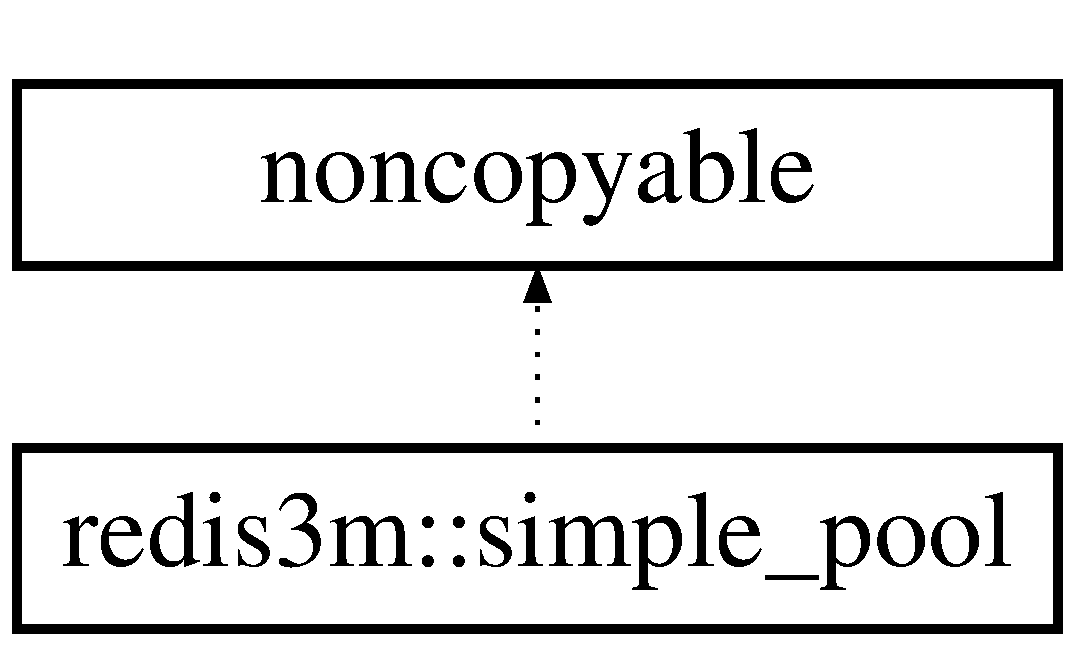
\includegraphics[height=2.000000cm]{classredis3m_1_1simple__pool}
\end{center}
\end{figure}
\subsection*{Public Types}
\begin{DoxyCompactItemize}
\item 
\hypertarget{classredis3m_1_1simple__pool_ab31a00132975f0a60479a1f8f6ad53de}{typedef boost\-::shared\-\_\-ptr\\*
$<$ \hyperlink{classredis3m_1_1simple__pool}{simple\-\_\-pool} $>$ {\bfseries ptr\-\_\-t}}\label{classredis3m_1_1simple__pool_ab31a00132975f0a60479a1f8f6ad53de}

\end{DoxyCompactItemize}
\subsection*{Public Member Functions}
\begin{DoxyCompactItemize}
\item 
\hypertarget{classredis3m_1_1simple__pool_ab0f7859a5bda82b92148856dddc472ca}{ptr\-\_\-t {\bfseries create} (const std\-::string \&host, unsigned int port)}\label{classredis3m_1_1simple__pool_ab0f7859a5bda82b92148856dddc472ca}

\item 
connection\-::ptr\-\_\-t \hyperlink{classredis3m_1_1simple__pool_a7aafd22508c1f113ca4b02f9eed211e3}{get} ()
\begin{DoxyCompactList}\small\item\em Get a working connection. \end{DoxyCompactList}\item 
void \hyperlink{classredis3m_1_1simple__pool_a385424b9f486990e455c16a6c949b5c0}{put} (connection\-::ptr\-\_\-t conn)
\begin{DoxyCompactList}\small\item\em Put back a connection for reuse. \end{DoxyCompactList}\item 
void \hyperlink{classredis3m_1_1simple__pool_ac0f6a8d1ff7a344a5b544b089e6d79c9}{set\-\_\-database} (unsigned int value)
\begin{DoxyCompactList}\small\item\em Set default database, all connection will be initialized selecting this database. \end{DoxyCompactList}\end{DoxyCompactItemize}


\subsection{Detailed Description}
Manages a pool of connections to a single Redis server. 

\subsection{Member Function Documentation}
\hypertarget{classredis3m_1_1simple__pool_a7aafd22508c1f113ca4b02f9eed211e3}{\index{redis3m\-::simple\-\_\-pool@{redis3m\-::simple\-\_\-pool}!get@{get}}
\index{get@{get}!redis3m::simple_pool@{redis3m\-::simple\-\_\-pool}}
\subsubsection[{get}]{\setlength{\rightskip}{0pt plus 5cm}connection\-::ptr\-\_\-t simple\-\_\-pool\-::get (
\begin{DoxyParamCaption}
{}
\end{DoxyParamCaption}
)}}\label{classredis3m_1_1simple__pool_a7aafd22508c1f113ca4b02f9eed211e3}


Get a working connection. 

\begin{DoxyReturn}{Returns}

\end{DoxyReturn}
\hypertarget{classredis3m_1_1simple__pool_a385424b9f486990e455c16a6c949b5c0}{\index{redis3m\-::simple\-\_\-pool@{redis3m\-::simple\-\_\-pool}!put@{put}}
\index{put@{put}!redis3m::simple_pool@{redis3m\-::simple\-\_\-pool}}
\subsubsection[{put}]{\setlength{\rightskip}{0pt plus 5cm}void simple\-\_\-pool\-::put (
\begin{DoxyParamCaption}
\item[{connection\-::ptr\-\_\-t}]{conn}
\end{DoxyParamCaption}
)}}\label{classredis3m_1_1simple__pool_a385424b9f486990e455c16a6c949b5c0}


Put back a connection for reuse. 


\begin{DoxyParams}{Parameters}
{\em conn} & \\
\hline
\end{DoxyParams}
\hypertarget{classredis3m_1_1simple__pool_ac0f6a8d1ff7a344a5b544b089e6d79c9}{\index{redis3m\-::simple\-\_\-pool@{redis3m\-::simple\-\_\-pool}!set\-\_\-database@{set\-\_\-database}}
\index{set\-\_\-database@{set\-\_\-database}!redis3m::simple_pool@{redis3m\-::simple\-\_\-pool}}
\subsubsection[{set\-\_\-database}]{\setlength{\rightskip}{0pt plus 5cm}void redis3m\-::simple\-\_\-pool\-::set\-\_\-database (
\begin{DoxyParamCaption}
\item[{unsigned int}]{value}
\end{DoxyParamCaption}
)\hspace{0.3cm}{\ttfamily [inline]}}}\label{classredis3m_1_1simple__pool_ac0f6a8d1ff7a344a5b544b089e6d79c9}


Set default database, all connection will be initialized selecting this database. 


\begin{DoxyParams}{Parameters}
{\em value} & \\
\hline
\end{DoxyParams}


The documentation for this class was generated from the following files\-:\begin{DoxyCompactItemize}
\item 
include/redis3m/simple\-\_\-pool.\-h\item 
src/simple\-\_\-pool.\-cpp\end{DoxyCompactItemize}

%--- End generated contents ---

% Index
\newpage
\phantomsection
\addcontentsline{toc}{chapter}{Index}
\printindex

\end{document}
